%% 
%% Copyright 2019-2024 Elsevier Ltd
%% 
%% Version 2.4
%% 
%% This file is part of the 'CAS Bundle'.
%% --------------------------------------
%% 
%% It may be distributed under the conditions of the LaTeX Project Public
%% License, either version 1.2 of this license or (at your option) any
%% later version.  The latest version of this license is in
%%    http://www.latex-project.org/lppl.txt
%% and version 1.2 or later is part of all distributions of LaTeX
%% version 1999/12/01 or later.
%% 
%% The list of all files belonging to the 'CAS Bundle' is
%% given in the file `manifest.txt'.
%% 
%% Template article for cas-dc documentclass for 
%% double column output.

%\documentclass[a4paper,fleqn,longmktitle]{cas-dc}
\documentclass[a4paper,fleqn]{cas-dc}

%\usepackage[authoryear,longnamesfirst]{natbib}
%\usepackage[authoryear]{natbib}
\usepackage[numbers]{natbib}

% Packages required by the numerical-methodology flowchart
\usepackage{tikz}
\usetikzlibrary{arrows.meta,positioning,shapes.geometric}
\usepackage{graphicx}
\usepackage{capt-of}
\graphicspath{{figs/}}
\usepackage{float}

%%%Author definitions
\def\tsc#1{\csdef{#1}{\textsc{\lowercase{#1}}\xspace}}
\tsc{WGM}
\tsc{QE}
\tsc{EP}
\tsc{PMS}
\tsc{BEC}
\tsc{DE}
%%%

\begin{document}
\let\WriteBookmarks\relax
\def\floatpagepagefraction{1}
\def\textpagefraction{.001}
\shorttitle{Leveraging social media news}
\shortauthors{J.K. Krishnan et~al.}

\title [mode = title]{This is a specimen $a_b$ title}                      
\tnotemark[1,2]

\tnotetext[1]{This document is the results of the research
	project funded by the National Science Foundation.}

\tnotetext[2]{The second title footnote which is a longer text matter
	to fill through the whole text width and overflow into
	another line in the footnotes area of the first page.}


\author[1,3]{J.K. Krishnan}[type=editor,
auid=000,bioid=1,
prefix=Sir,
role=Researcher,
orcid=0000-0001-0000-0000]
\cormark[1]
\fnmark[1]
\ead{jkk@example.in}
\ead[url]{www.jkkrishnan.in}

\credit{Conceptualization of this study, Methodology, Software}

%\address[1]{, Street 129, 1043 NX Amsterdam, The Netherlands}
\affiliation[1]{organization={Department of Physics, J.K. Institute of Science},
	addressline={Jawahar Nagar}, 
	city={Trivandrum},
	%               citysep={}, % Uncomment if no comma needed between city and postcode
	postcode={695013}, 
	state={Kerala},
	country={India}}

\author[2,4]{Han Thane}[style=chinese]

\author[2,3]{William {J. Hansen}}[%
role=Co-ordinator,
suffix=Jr,
]
\fnmark[2]
\ead{wjh@example.org}
\ead[URL]{https://www.university.org}

\credit{Data curation, Writing - Original draft preparation}

\affiliation[2]{organization={World Scientific University},
	addressline={Street 29}, 
	postcode={1011 NX}, 
	postcodesep={}, 
	city={Amsterdam},
	country={The Netherlands}}

\author[1,3]{T. Rafeeq}
\cormark[2]
\fnmark[1,3]
\ead{t.rafeeq@example.in}
\ead[URL]{www.campus.in}

\affiliation[3]{organization={University of Intelligent Studies},
	addressline={Street 15}, 
	city={Jabaldesh},
	postcode={825001}, 
	state={Orissa}, 
	country={India}}

\cortext[cor1]{Corresponding author}
\cortext[cor2]{Principal corresponding author}
\fntext[fn1]{This is the first author footnote, but is common to third
	author as well.}
\fntext[fn2]{Another author footnote, this is a very long footnote and
	it should be a really long footnote. But this footnote is not yet
	sufficiently long enough to make two lines of footnote text.}

\nonumnote{This note has no numbers. In this work we demonstrate $a_b$
	the formation Y\_1 of a new type of polariton on the interface
	between a cuprous oxide slab and a polystyrene micro-sphere placed
	on the slab.
}

\begin{abstract}
	This template helps you to create a properly formatted \LaTeX\ manuscript.
	
	\noindent\texttt{\textbackslash begin{abstract}} \dots 
	\texttt{\textbackslash end{abstract}} and
	\verb+\begin{keyword}+ \verb+...+ \verb+\end{keyword}+ 
	which
	contain the abstract and keywords respectively. 
	
	\noindent Each keyword shall be separated by a \verb+\sep+ command.
\end{abstract}

\begin{graphicalabstract}
	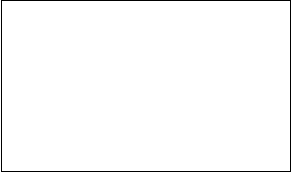
\includegraphics{figs/cas-grabs.pdf}
\end{graphicalabstract}

\begin{highlights}
	\item Research highlights item 1
	\item Research highlights item 2
	\item Research highlights item 3
\end{highlights}

\begin{keywords}
	quadrupole exciton \sep polariton \sep \WGM \sep \BEC
\end{keywords}


\maketitle

\section{Introduction}

The Elsevier cas-dc class is based on the
standard article class and supports almost all of the functionality of
that class. In addition, it features commands and options to format the
\begin{itemize} \item document style \item baselineskip \item front
	matter \item keywords and MSC codes \item theorems, definitions and
	proofs \item lables of enumerations \item citation style and labeling.
\end{itemize}

This class depends on the following packages
for its proper functioning:

\begin{enumerate}
	\itemsep=0pt
	\item {natbib.sty} for citation processing;
	\item {geometry.sty} for margin settings;
	\item {fleqn.clo} for left aligned equations;
	\item {graphicx.sty} for graphics inclusion;
	\item {hyperref.sty} optional packages if hyperlinking is
	required in the document;
\end{enumerate}  

All the above packages are part of any
standard \LaTeX{} installation.
Therefore, the users need not be
bothered about downloading any extra packages.

% ============================================================
% NUMERICAL METHODOLOGY — updated manuscript section
% ============================================================
\section{Numerical methodology}
\label{sec:numerical_methodology}


% ============================================================
% OVERALL NUMERICAL FRAMEWORK
% ============================================================

\subsection{Overall numerical framework}
\label{subsec:overall_framework}

A two-dimensional steady aero--hydraulic framework was developed to
evaluate the aerodynamic behaviour of airfoils containing passive
internal channels. The external flow is modelled using an
incompressible, inviscid and irrotational source--vortex panel method,
while the pressure-driven flow through each internal passage is
described using the Hagen--Poiseuille and Darcy--Weisbach relations for
circular channels. The two models are coupled through the pressure and
surface-normal velocity at the channel openings.

The external aerodynamic solution determines the pressure difference
between the two openings of each channel. This pressure difference
drives the internal flow, which subsequently modifies the aerodynamic
boundary condition through a surface-normal transpiration velocity.
The external pressure field and internal channel flow are therefore
determined as a coupled aero--hydraulic system.

The calculation is initialised using an impermeable-airfoil solution,
for which the surface-normal transpiration velocity is set to zero.
The resulting surface pressures provide the initial pressure differences
across the internal passages and, consequently, the initial estimates
of the channel flow rates. The aerodynamic and hydraulic solutions are
then coupled until a consistent pressure and channel-flow solution is
obtained. Converged solutions are retained for aerodynamic and
internal-flow analysis, whereas non-converged cases are reported as
\texttt{NaN}.

The external aerodynamic formulation assumes steady, incompressible,
inviscid and irrotational flow. Consequently, boundary-layer
development, skin-friction drag, flow separation and stall are not
resolved. The predicted drag coefficient therefore represents only the
pressure-drag contribution obtained from the potential-flow solution.

The numerical procedure is summarised in
Fig.~\ref{fig:coupled_iteration_loop}.


\begin{figure}
	\centering
	
	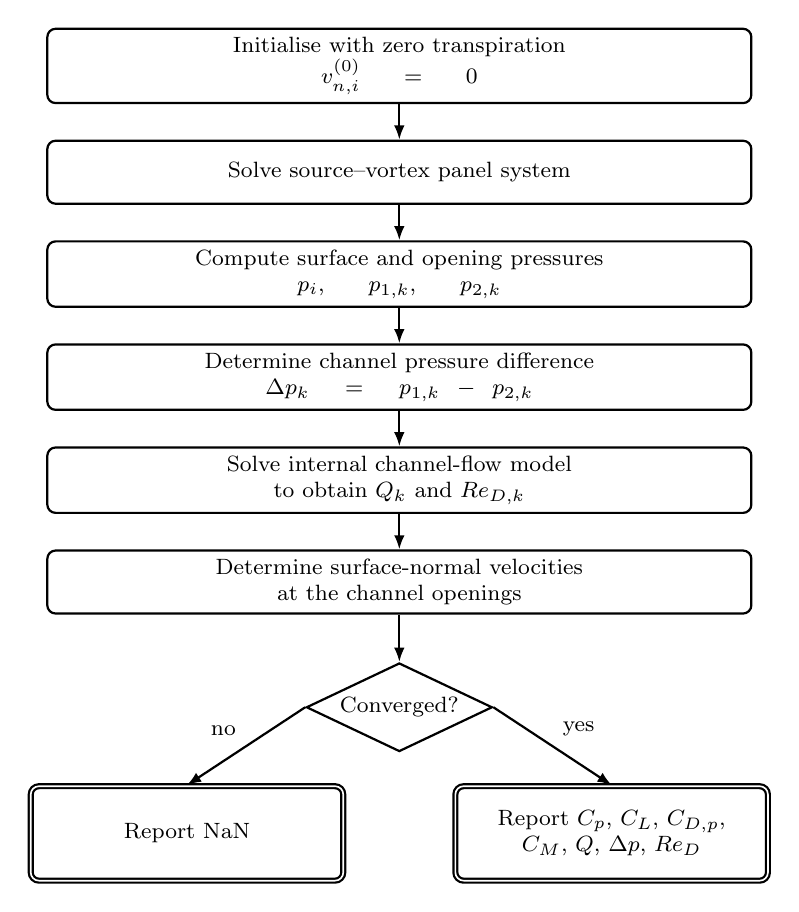
\begin{tikzpicture}[
		node distance=4.5mm,
		process/.style={
			rectangle,
			draw,
			rounded corners=3pt,
			thick,
			align=center,
			text width=0.72\linewidth,
			minimum height=8mm,
			inner sep=3pt,
			font=\footnotesize
		},
		decision/.style={
			diamond,
			draw,
			thick,
			align=center,
			aspect=2.1,
			inner sep=1.5pt,
			font=\footnotesize
		},
		output/.style={
			rectangle,
			draw,
			double,
			rounded corners=3pt,
			thick,
			align=center,
			text width=0.31\linewidth,
			minimum height=12mm,
			inner sep=3pt,
			font=\footnotesize
		},
		arrow/.style={
			-{Latex[length=1.8mm]},
			thick
		}
		]
		
		\node[process] (init)
		{Initialise with zero transpiration\\
			$v_{n,i}^{(0)}=0$};
		
		\node[process, below=of init] (panel)
		{Solve source--vortex panel system};
		
		\node[process, below=of panel] (pressure)
		{Compute surface and opening pressures\\
			$p_i,\;p_{1,k},\;p_{2,k}$};
		
		\node[process, below=of pressure] (dp)
		{Determine channel pressure difference\\
			$\Delta p_k=p_{1,k}-p_{2,k}$};
		
		\node[process, below=of dp] (flow)
		{Solve internal channel-flow model\\
			to obtain $Q_k$ and $Re_{D,k}$};
		
		\node[process, below=of flow] (update)
		{Determine surface-normal velocities\\
			at the channel openings};
		
		\node[decision, below=6mm of update] (converged)
		{Converged?};
		
		\node[output, below left=7mm and 1mm of converged] (nan)
		{Report NaN};
		
		\node[output, below right=7mm and 1mm of converged] (results)
		{Report $C_p$, $C_L$, $C_{D,p}$,\\
			$C_M$, $Q$, $\Delta p$, $Re_D$};
		
		\draw[arrow] (init) -- (panel);
		\draw[arrow] (panel) -- (pressure);
		\draw[arrow] (pressure) -- (dp);
		\draw[arrow] (dp) -- (flow);
		\draw[arrow] (flow) -- (update);
		\draw[arrow] (update) -- (converged);
		
		\draw[arrow]
		(converged.west)
		-- node[above left,font=\footnotesize] {no}
		(nan.north);
		
		\draw[arrow]
		(converged.east)
		-- node[above right,font=\footnotesize] {yes}
		(results.north);
		
	\end{tikzpicture}
	
	\caption{Coupled aero--hydraulic solution procedure.}
	\label{fig:coupled_iteration_loop}
\end{figure}


% ============================================================
% GEOMETRY
% ============================================================

\subsection{Airfoil geometry and porous configurations}
\label{subsec:airfoil_porous_geometry}

The baseline geometry is a NACA~0018 airfoil with chord $c$. The
NACA four-digit coordinates are generated analytically and discretised
using cosine spacing along the chord, providing increased panel density
near the leading and trailing edges.

Each aerodynamic panel $i$ is characterised by its length $S_i$,
control point $(x_i,y_i)$, unit tangent vector

\begin{equation}
	\boldsymbol{t}_i
	=
	(t_{x,i},t_{y,i}),
\end{equation}

and outward unit normal vector

\begin{equation}
	\boldsymbol{n}_i
	=
	(n_{x,i},n_{y,i}).
\end{equation}

The porous structure is represented by passive circular channels
connecting pairs of openings on the airfoil surface. No prescribed
mass-flow rate or external pumping mechanism is imposed. Instead, the
magnitude and direction of the internal flow are determined entirely
by the aerodynamic pressure difference between the two surface
openings.

Three porous configurations are considered:

\begin{enumerate}
	
	\item \textbf{Horizontal model (M1):}
	four independent chordwise passages, with two channels located above
	and two below the chord line. Both openings of each passage are
	located on the same airfoil surface.
	
	\item \textbf{Vertical model (M2):}
	four independent lower-to-upper passages distributed between
	$x/c=0.1$ and $x/c=0.9$.
	
	\item \textbf{Combined independent model (M3):}
	the horizontal and vertical passages are superposed, resulting in
	eight internal passages. The passages remain hydraulically
	independent, and geometrical intersections do not represent
	connected internal junctions.
	
\end{enumerate}

The three porous-airfoil configurations considered in the present
study are illustrated in Fig.~\ref{fig:porous_models}.


\begin{figure}
	\centering
	
	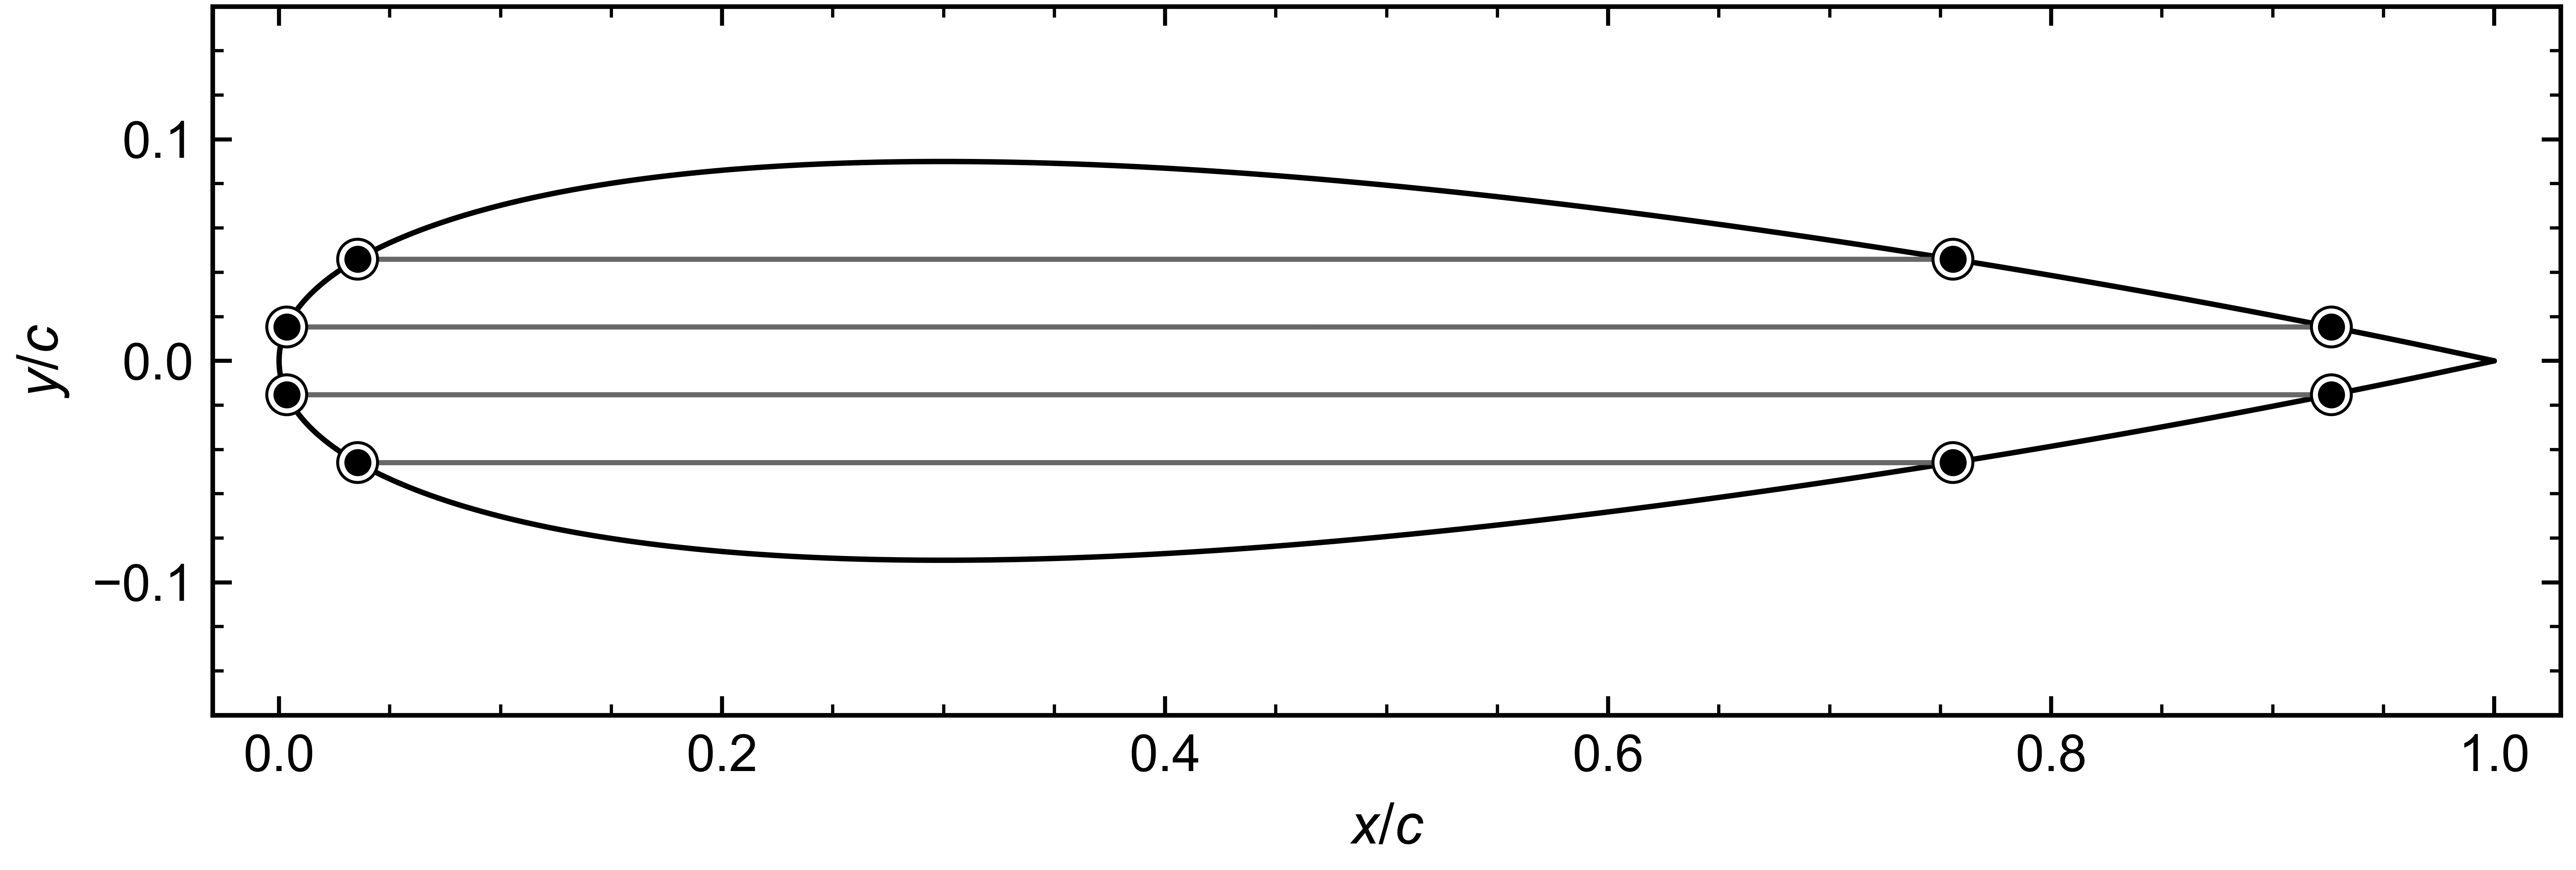
\includegraphics[width=0.85\columnwidth]
	{figs/model1_horizontal.png}
	
	\vspace{1mm}
	
	{\small \textbf{(a)} Horizontal model (M1)}
	
	\vspace{3mm}
	
	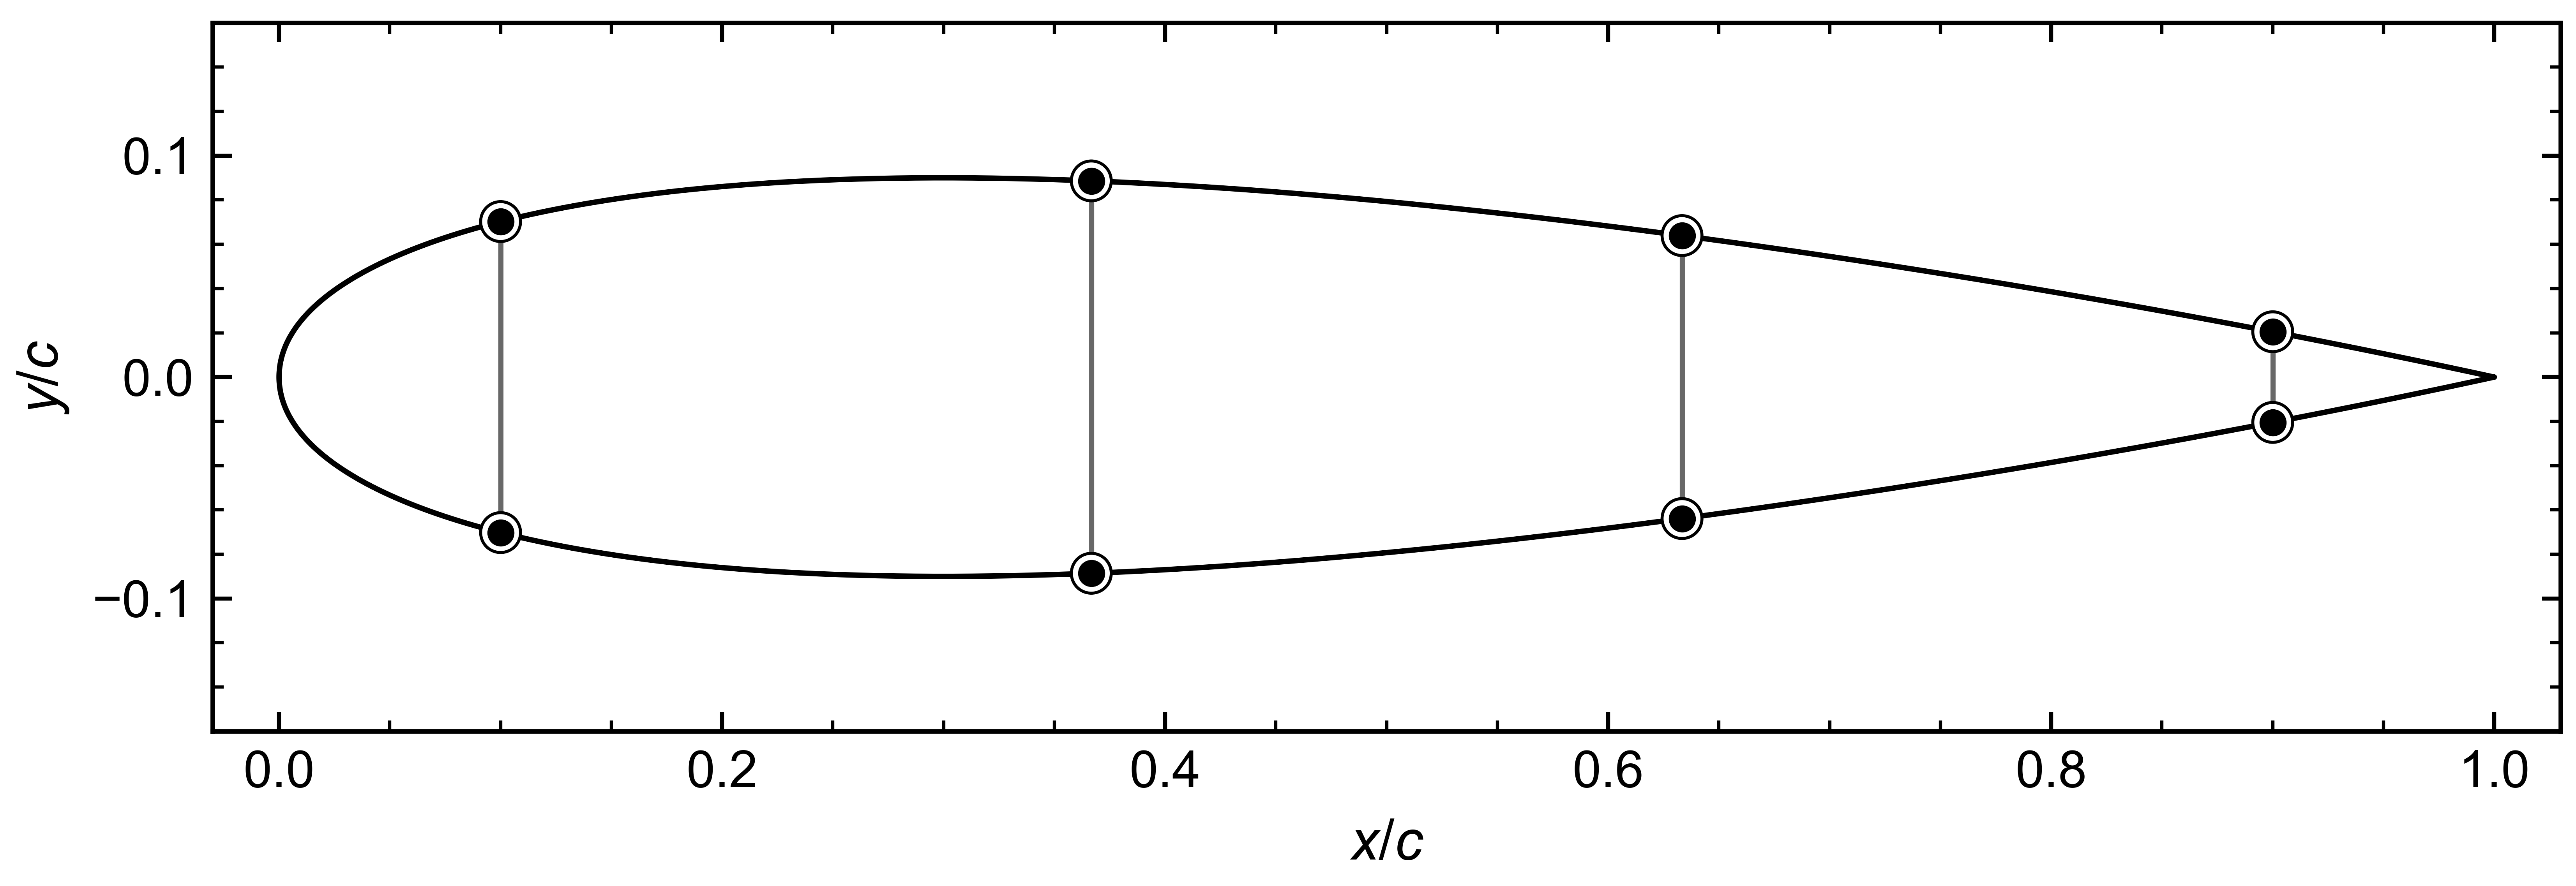
\includegraphics[width=0.85\columnwidth]
	{figs/model2_vertical.png}
	
	\vspace{1mm}
	
	{\small \textbf{(b)} Vertical model (M2)}
	
	\vspace{3mm}
	
	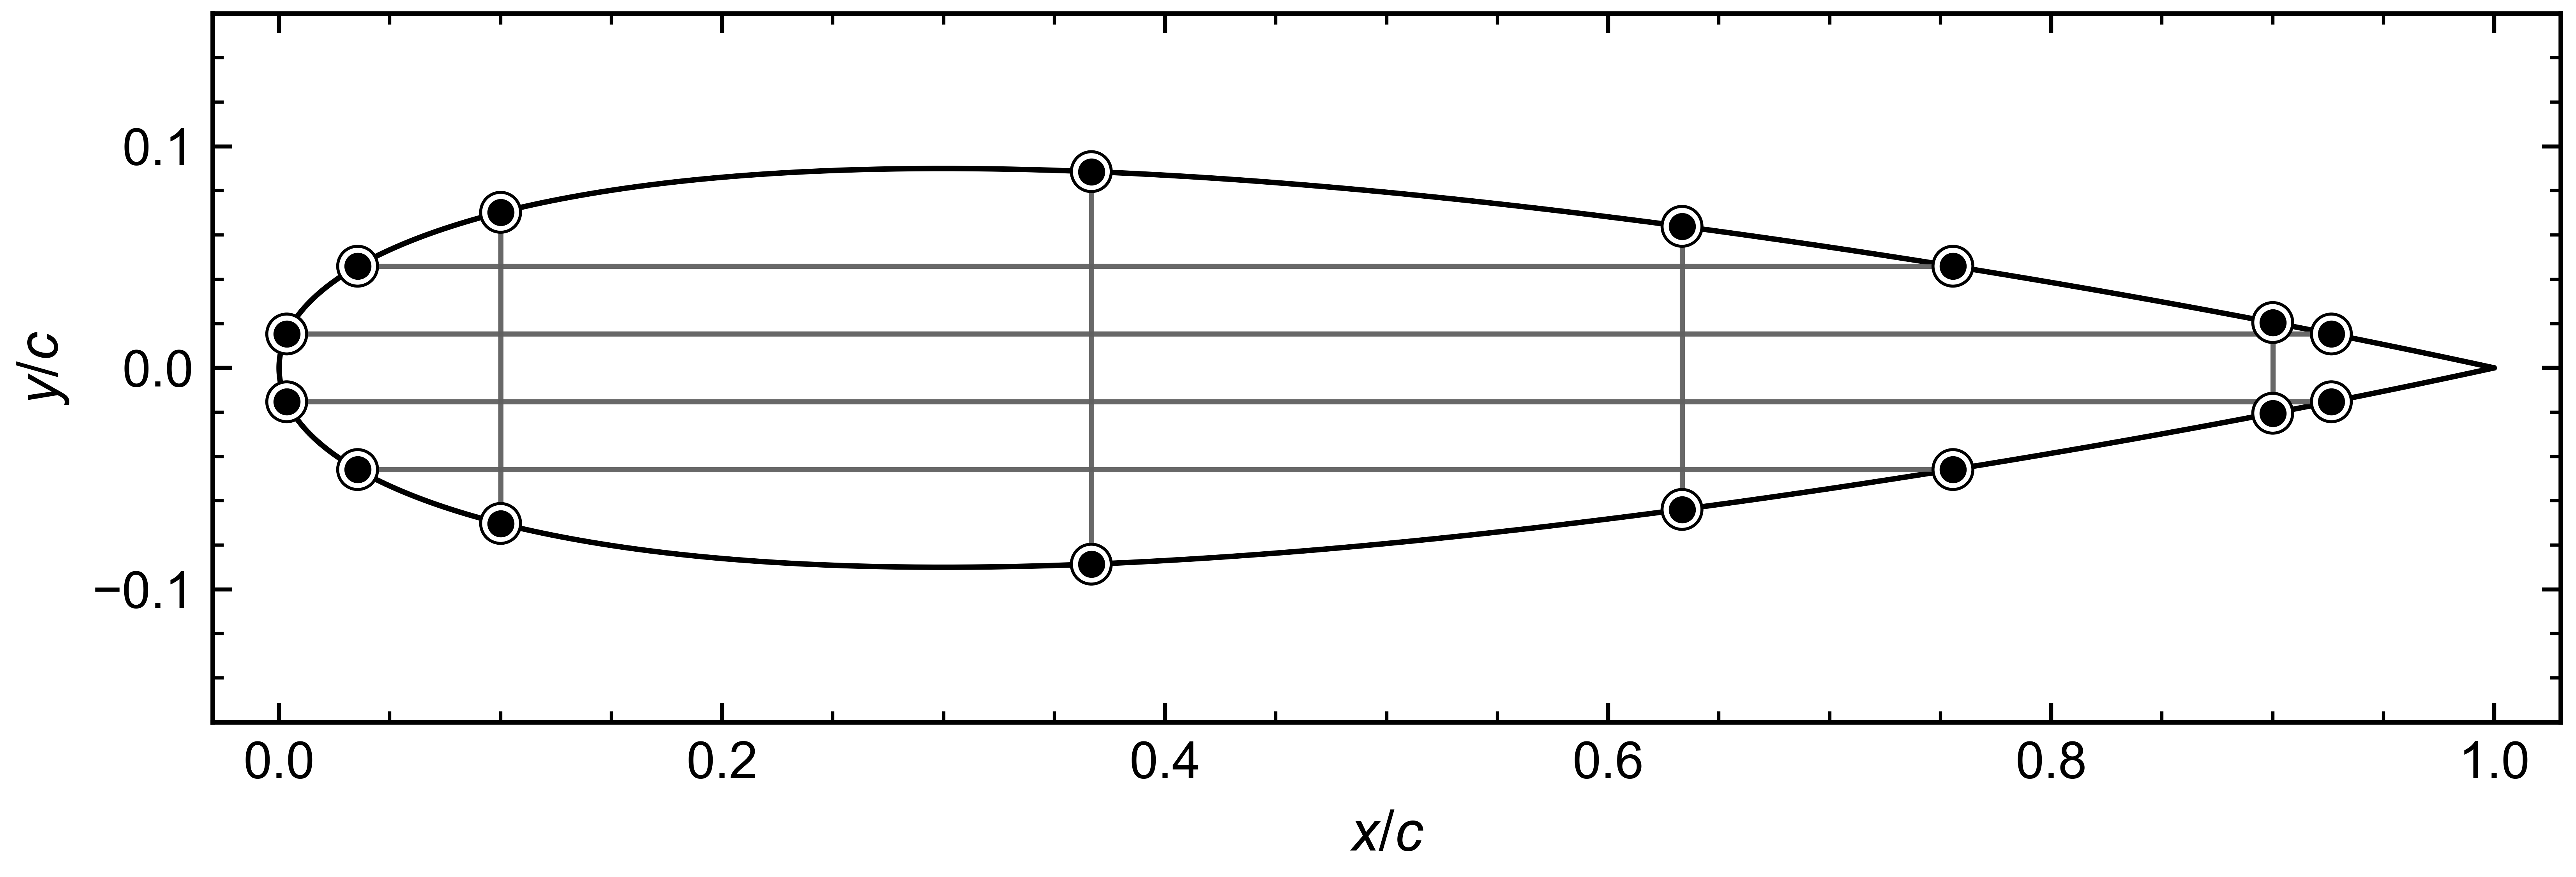
\includegraphics[width=0.85\columnwidth]
	{figs/model3_combined.png}
	
	\vspace{1mm}
	
	{\small \textbf{(c)} Combined independent model (M3)}
	
	\caption{
		Porous-airfoil configurations considered in the present study:
		(a) horizontal model (M1),
		(b) vertical model (M2), and
		(c) combined independent model (M3).
	}
	\label{fig:porous_models}
\end{figure}


The positions of the surface openings are obtained by interpolation of
the upper and lower airfoil surfaces rather than by restricting their
locations to panel control points. This preserves the prescribed
orientation and position of the internal passages independently of the
aerodynamic panel resolution.

The channel geometry is checked before the coupled calculation to
ensure that the openings remain within the permitted chordwise region,
do not overlap, fit within the local airfoil thickness and satisfy the
specified minimum separation.

Each passage $k$ is characterised by a diameter $D_k$ and a
centreline length $L_k$. The channel length is determined from the
geometry of the two corresponding surface openings and the internal
passage connecting them.


% ============================================================
% EXTERNAL AERODYNAMIC MODEL
% ============================================================

\subsection{External aerodynamic model}
\label{subsec:external_aerodynamic_model}


\subsubsection{Potential-flow formulation}

The external flow is assumed to be incompressible, inviscid and
irrotational. The velocity field can therefore be expressed in terms
of a scalar velocity potential,

\begin{equation}
	\boldsymbol{V}
	=
	\nabla\Phi.
\end{equation}

Application of mass conservation gives Laplace's equation,

\begin{equation}
	\nabla^2\Phi
	=
	0.
	\label{eq:laplace}
\end{equation}

The numerical solution is constructed by superposing the uniform
freestream with constant-strength source distributions over the
airfoil surface and a single constant vortex strength distributed
around the complete airfoil boundary. The source distributions
represent the airfoil thickness, while the global vortex strength
introduces the circulation required to generate lift.


\subsubsection{Source--vortex panel formulation}

For an airfoil discretised into $N$ panels, the aerodynamic unknowns
are the $N$ source strengths

\begin{equation}
	\boldsymbol{\lambda}
	=
	\left[
	\lambda_1,\lambda_2,\ldots,\lambda_N
	\right]^{\mathrm T}
\end{equation}

and the global vortex strength $\gamma$.

The normal and tangential source influence coefficients are denoted by
$I_{ij}$ and $J_{ij}$, respectively, while $K_{ij}$ and $L_{ij}$
represent the corresponding vortex influence coefficients.

For an impermeable airfoil, the normal velocity at every control point
is zero. To represent a porous opening, this condition is modified by
prescribing a surface-normal transpiration velocity $v_{n,i}$,

\begin{equation}
	\boldsymbol{V}_i
	\cdot
	\boldsymbol{n}_i
	=
	v_{n,i}.
	\label{eq:porous_normal_bc}
\end{equation}

The conventional impermeable boundary condition is recovered when

\begin{equation}
	v_{n,i}=0.
\end{equation}

Following discretisation, the normal boundary condition for panel $i$
becomes

\begin{equation}
	\pi\lambda_i
	+
	\sum_{\substack{j=1\\j\neq i}}^{N}
	I_{ij}\lambda_j
	-
	\gamma
	\sum_{j=1}^{N}K_{ij}
	=
	-2\pi V_{\infty}\cos\beta_i
	+
	2\pi v_{n,i},
	\label{eq:normal_panel_equation}
\end{equation}

where $\beta_i$ denotes the angle between the local panel normal and
the freestream direction.

The trailing-edge Kutta condition is imposed by requiring the
tangential velocities on the first and final panels to be equal in
magnitude and opposite in direction,

\begin{equation}
	V_{t,1}
	+
	V_{t,N}
	=
	0.
	\label{eq:kutta}
\end{equation}

The $N$ normal boundary conditions together with the Kutta condition
produce an $(N+1)\times(N+1)$ linear system,

\begin{equation}
	\begin{bmatrix}
		\boldsymbol{A}_{\lambda}
		&
		\boldsymbol{a}_{\gamma}
		\\
		\boldsymbol{a}_{K}^{\mathrm T}
		&
		a_{K,\gamma}
	\end{bmatrix}
	\begin{bmatrix}
		\boldsymbol{\lambda}\\
		\gamma
	\end{bmatrix}
	=
	\begin{bmatrix}
		\boldsymbol{b}(\boldsymbol v_n)\\
		b_K
	\end{bmatrix}.
	\label{eq:panel_matrix}
\end{equation}

The influence matrix depends only on the discretised airfoil geometry.
It is therefore assembled and LU-factorised once for each geometry,
while the right-hand side is updated according to the freestream
condition and surface-normal transpiration velocity.


\subsubsection{Surface velocity and pressure}

Following solution of the panel system, the tangential velocity on
panel $i$ is evaluated as

\begin{equation}
	V_{t,i}
	=
	V_{\infty}\sin\beta_i
	+
	\frac{1}{2\pi}
	\sum_{j=1}^{N}\lambda_jJ_{ij}
	+
	\frac{\gamma}{2}
	-
	\frac{\gamma}{2\pi}
	\sum_{j=1}^{N}L_{ij}.
	\label{eq:tangential_velocity}
\end{equation}

At a porous opening, the local surface velocity contains both
tangential and normal components. The velocity magnitude is therefore

\begin{equation}
	V_i^2
	=
	V_{t,i}^{2}
	+
	v_{n,i}^{2}.
	\label{eq:surface_velocity_magnitude}
\end{equation}

The pressure coefficient is obtained from the steady incompressible
Bernoulli equation,

\begin{equation}
	C_{p,i}
	=
	1-
	\frac{
		V_{t,i}^{2}
		+
		v_{n,i}^{2}}
	{V_{\infty}^{2}}.
	\label{eq:pressure_coefficient}
\end{equation}

The corresponding absolute pressure is

\begin{equation}
	p_i
	=
	p_{\infty}
	+
	\frac{1}{2}
	\rho_{\infty}
	V_{\infty}^{2}
	C_{p,i}.
	\label{eq:absolute_pressure}
\end{equation}


% ============================================================
% INTERNAL FLOW MODEL
% ============================================================

\subsection{Internal channel-flow model}
\label{subsec:internal_channel_flow}

The internal flow through each porous passage is modelled as
pressure-driven flow through a circular channel. For channel $k$ with
diameter $D_k$, the cross-sectional area is

\begin{equation}
	A_k
	=
	\frac{\pi D_k^2}{4}.
	\label{eq:channel_area}
\end{equation}

The mean internal velocity is related to the volumetric flow rate by

\begin{equation}
	\overline{U}_k
	=
	\frac{Q_k}{A_k},
	\label{eq:mean_channel_velocity}
\end{equation}

where $Q_k~[\mathrm{m^3\,s^{-1}}]$ is the volumetric flow rate
through the channel.

The internal flow is driven by the pressure difference between the two
surface openings,

\begin{equation}
	\Delta p_k
	=
	p_{1,k}
	-
	p_{2,k}.
	\label{eq:channel_pressure_difference}
\end{equation}

The sign of $\Delta p_k$ determines the direction of the internal
flow. The corresponding channel Reynolds number is

\begin{equation}
	Re_{D,k}
	=
	\frac{
		\rho_{\infty}
		|\overline{U}_k|
		D_k}
	{\mu_{\infty}}.
	\label{eq:internal_reynolds}
\end{equation}

For fully developed laminar flow through a circular channel, the
pressure-driven flow is described by the Hagen--Poiseuille equation,

\begin{equation}
	Q_k
	=
	\frac{
		\pi D_k^4}
	{128\mu_{\infty}L_k}
	\Delta p_k.
	\label{eq:hagen_poiseuille}
\end{equation}

This formulation naturally accounts for the direction of flow through
the sign of $\Delta p_k$.

The pressure loss can equivalently be expressed using the
Darcy--Weisbach relation,

\begin{equation}
	|\Delta p_k|
	=
	f_k
	\frac{L_k}{D_k}
	\frac{
		\rho_{\infty}
		\overline{U}_k^2}
	{2},
	\label{eq:darcy_weisbach}
\end{equation}

where $f_k$ is the Darcy friction factor.

For fully developed laminar flow through a circular pipe,

\begin{equation}
	f_{\mathrm{lam},k}
	=
	\frac{64}{Re_{D,k}}.
	\label{eq:laminar_friction_factor}
\end{equation}

The Hagen--Poiseuille and Darcy--Weisbach formulations are therefore
equivalent for fully developed laminar flow through the circular
channels considered here.


% ============================================================
% COUPLING
% ============================================================

\subsection{Aero--hydraulic coupling}
\label{subsec:aero_hydraulic_coupling}

The aerodynamic and internal-flow models are coupled through the
pressure and surface-normal velocity at the channel openings.

The pressure at each channel opening is obtained from the aerodynamic
surface-pressure distribution. When an opening intersects multiple
panels, its pressure is evaluated using a length-weighted average over
the corresponding surface footprint. For opening $m$ of channel $k$,

\begin{equation}
	p_{m,k}
	=
	\frac{
		\displaystyle
		\sum_{i\in\mathcal{P}_{m,k}}
		p_i\ell_i}
	{
		\displaystyle
		\sum_{i\in\mathcal{P}_{m,k}}
		\ell_i},
	\qquad
	m=1,2,
	\label{eq:opening_pressure}
\end{equation}

where $\mathcal{P}_{m,k}$ denotes the set of panels intersected by the
opening and $\ell_i$ is the corresponding overlap length.

The two opening pressures provide the channel pressure difference,

\begin{equation}
	\Delta p_k
	=
	p_{1,k}
	-
	p_{2,k},
\end{equation}

which is supplied to the internal-flow model to determine $Q_k$.

The mean velocity through each circular opening is

\begin{equation}
	U_{\mathrm{open},k}
	=
	\frac{Q_k}{A_k}.
	\label{eq:opening_velocity}
\end{equation}

This velocity is imposed on the external aerodynamic model as a
surface-normal transpiration velocity. With the outward panel normal
defined as positive, flow entering the airfoil is assigned a negative
normal velocity, whereas flow leaving the airfoil is assigned a
positive normal velocity,

\begin{equation}
	v_{n,k}^{\mathrm{in}}
	=
	-\frac{Q_k}{A_k},
	\qquad
	v_{n,k}^{\mathrm{out}}
	=
	+\frac{Q_k}{A_k}.
	\label{eq:opening_transpiration}
\end{equation}

When an opening intersects multiple aerodynamic panels, the prescribed
normal velocity is applied over the corresponding opening footprint so
that the transpiration boundary condition is represented consistently
by the discretised airfoil surface.

The updated surface-normal velocity modifies the panel-method boundary
condition and therefore changes the external pressure distribution.
The new opening pressures are subsequently supplied to the
internal-flow model, and the aerodynamic and hydraulic solutions are
coupled until the channel flow used to impose the opening velocity is
consistent with that predicted from the resulting pressure difference.

A case is classified as converged when the prescribed coupling
criterion is satisfied for all channels. Cases that do not satisfy the
convergence requirement are reported as \texttt{NaN}.


% ============================================================
% AERODYNAMIC COEFFICIENTS
% ============================================================

\subsection{Aerodynamic coefficients}
\label{subsec:aerodynamic_coefficients}

The aerodynamic forces are obtained by integrating the pressure
contribution over the discretised airfoil surface. The contribution of
panel $i$ to the global Cartesian force coefficients is

\begin{align}
	\mathrm d C_{x,i}
	&=
	-C_{p,i}
	n_{x,i}
	\frac{S_i}{c},
	\label{eq:dcx}\\
	\mathrm d C_{y,i}
	&=
	-C_{p,i}
	n_{y,i}
	\frac{S_i}{c}.
	\label{eq:dcy}
\end{align}

The total Cartesian force coefficients are

\begin{equation}
	C_x
	=
	\sum_{i=1}^{N}
	\mathrm d C_{x,i},
	\qquad
	C_y
	=
	\sum_{i=1}^{N}
	\mathrm d C_{y,i}.
\end{equation}

Rotation into the freestream-aligned coordinate system gives the lift
and pressure-drag coefficients,

\begin{align}
	C_L
	&=
	C_y\cos\alpha
	-
	C_x\sin\alpha,
	\label{eq:cl}\\
	C_{D,p}
	&=
	C_x\cos\alpha
	+
	C_y\sin\alpha.
	\label{eq:cd}
\end{align}

The pitching-moment coefficient is evaluated about the quarter-chord
reference location,

\begin{equation}
	(x_{\mathrm{ref}},y_{\mathrm{ref}})
	=
	(0.25c,0),
\end{equation}

using

\begin{equation}
	C_M
	=
	-\sum_{i=1}^{N}
	\frac{
		(x_i-x_{\mathrm{ref}})
		\mathrm d C_{y,i}
		-
		(y_i-y_{\mathrm{ref}})
		\mathrm d C_{x,i}}
	{c}.
	\label{eq:cm}
\end{equation}

For diagnostic comparison, an additional lift coefficient is
calculated from the solved circulation using the Kutta--Joukowski
relationship,

\begin{equation}
	C_{L,\Gamma}
	=
	\frac{
		2\gamma
		\displaystyle\sum_{i=1}^{N}S_i}
	{V_{\infty}c}.
	\label{eq:kutta_joukowski_lift}
\end{equation}


% ============================================================
% NUMERICAL SETUP
% ============================================================

\subsection{Numerical setup}
\label{subsec:numerical_setup}

The aerodynamic response of each porous configuration is evaluated
relative to an impermeable reference airfoil using the same geometry,
panel discretisation and operating conditions. An inviscid XFOIL
solution may additionally be used for comparison of the
impermeable-airfoil pressure distribution and angle-of-attack response.

Unless otherwise stated, the calculations are performed for a
NACA~0018 airfoil with chord

\begin{equation}
	c
	=
	1~\mathrm{m},
\end{equation}

discretised using $N=1000$ panels.

The freestream fluid properties are

\begin{equation}
	\rho_{\infty}
	=
	1.225~\mathrm{kg\,m^{-3}},
\end{equation}

\begin{equation}
	\mu_{\infty}
	=
	1.8\times10^{-5}~\mathrm{Pa\,s},
\end{equation}

and

\begin{equation}
	p_{\infty}
	=
	101325~\mathrm{Pa}.
\end{equation}

A chord Reynolds number of

\begin{equation}
	Re_c
	=
	5.0\times10^5
\end{equation}

is prescribed.

The corresponding freestream velocity is calculated from

\begin{equation}
	V_{\infty}
	=
	\frac{
		Re_c\mu_{\infty}}
	{\rho_{\infty}c}.
	\label{eq:freestream_velocity}
\end{equation}

The principal fixed-angle analysis is performed at

\begin{equation}
	\alpha
	=
	4^\circ.
\end{equation}

The angle-of-attack sweep extends from $-5^\circ$ to $15^\circ$ in
increments of $1^\circ$.

Circular channel diameters of

\begin{equation}
	D
	=
	8,\;9,\;\text{and}\;10~\mathrm{mm}
\end{equation}

are considered.

Each angle of attack is solved independently, and the solution from the
preceding angle is not used to initialise the subsequent case.
% ============================================================
% END NUMERICAL METHODOLOGY
% ============================================================
% ============================================================
% RESULTS
% ============================================================

% ============================================================
% RESULTS AND DISCUSSION
% ============================================================

\section{Results and discussion}
\label{sec:results_discussion}

The aerodynamic response of the three porous-airfoil configurations was
investigated over an angle-of-attack range of $-5^\circ$ to
$15^\circ$. Three circular-channel diameters,
$D=8$, $9$ and $10~\mathrm{mm}$, were considered for the horizontal
(M1), vertical (M2) and combined horizontal--vertical (M3)
configurations. The corresponding impermeable panel-method solution
and the inviscid XFOIL prediction are included as reference cases.

The influence of the porous channels is first assessed using the
integrated lift and pitching-moment coefficients. The resulting
aerodynamic trends are then related to changes in the external pressure
and velocity fields. The flow-field comparison is presented for
$\alpha=10^\circ$ and $D=9~\mathrm{mm}$.


% ============================================================
% BASELINE VALIDATION
% ============================================================

\subsection{Baseline aerodynamic validation}
\label{subsec:baseline_validation}

The impermeable source--vortex panel solution is compared with the
corresponding inviscid XFOIL prediction in
Figs.~\ref{fig:cl_aoa_three_models} and
\ref{fig:cm_aoa_three_models}. The two approaches show similar
angle-of-attack trends for both lift and pitching moment over the
investigated range.

The agreement between the two impermeable-airfoil solutions provides
a reference for evaluating the aerodynamic changes introduced by the
internal channels. Small differences between the panel-method and
XFOIL predictions are expected because the two methods employ
different numerical formulations, although both represent inviscid
external flow.

The impermeable panel solution is therefore used as the primary
reference when evaluating the effect of the porous configurations,
ensuring that the porous and solid cases are compared using the same
panel discretisation and aerodynamic formulation.


% ============================================================
% LIFT
% ============================================================

\subsection{Effect of porous-channel configuration on lift}
\label{subsec:lift_results}

Figure~\ref{fig:cl_aoa_three_models} compares the variation of lift
coefficient with angle of attack for the three porous configurations
and channel diameters.

\begin{figure*}
	\centering
	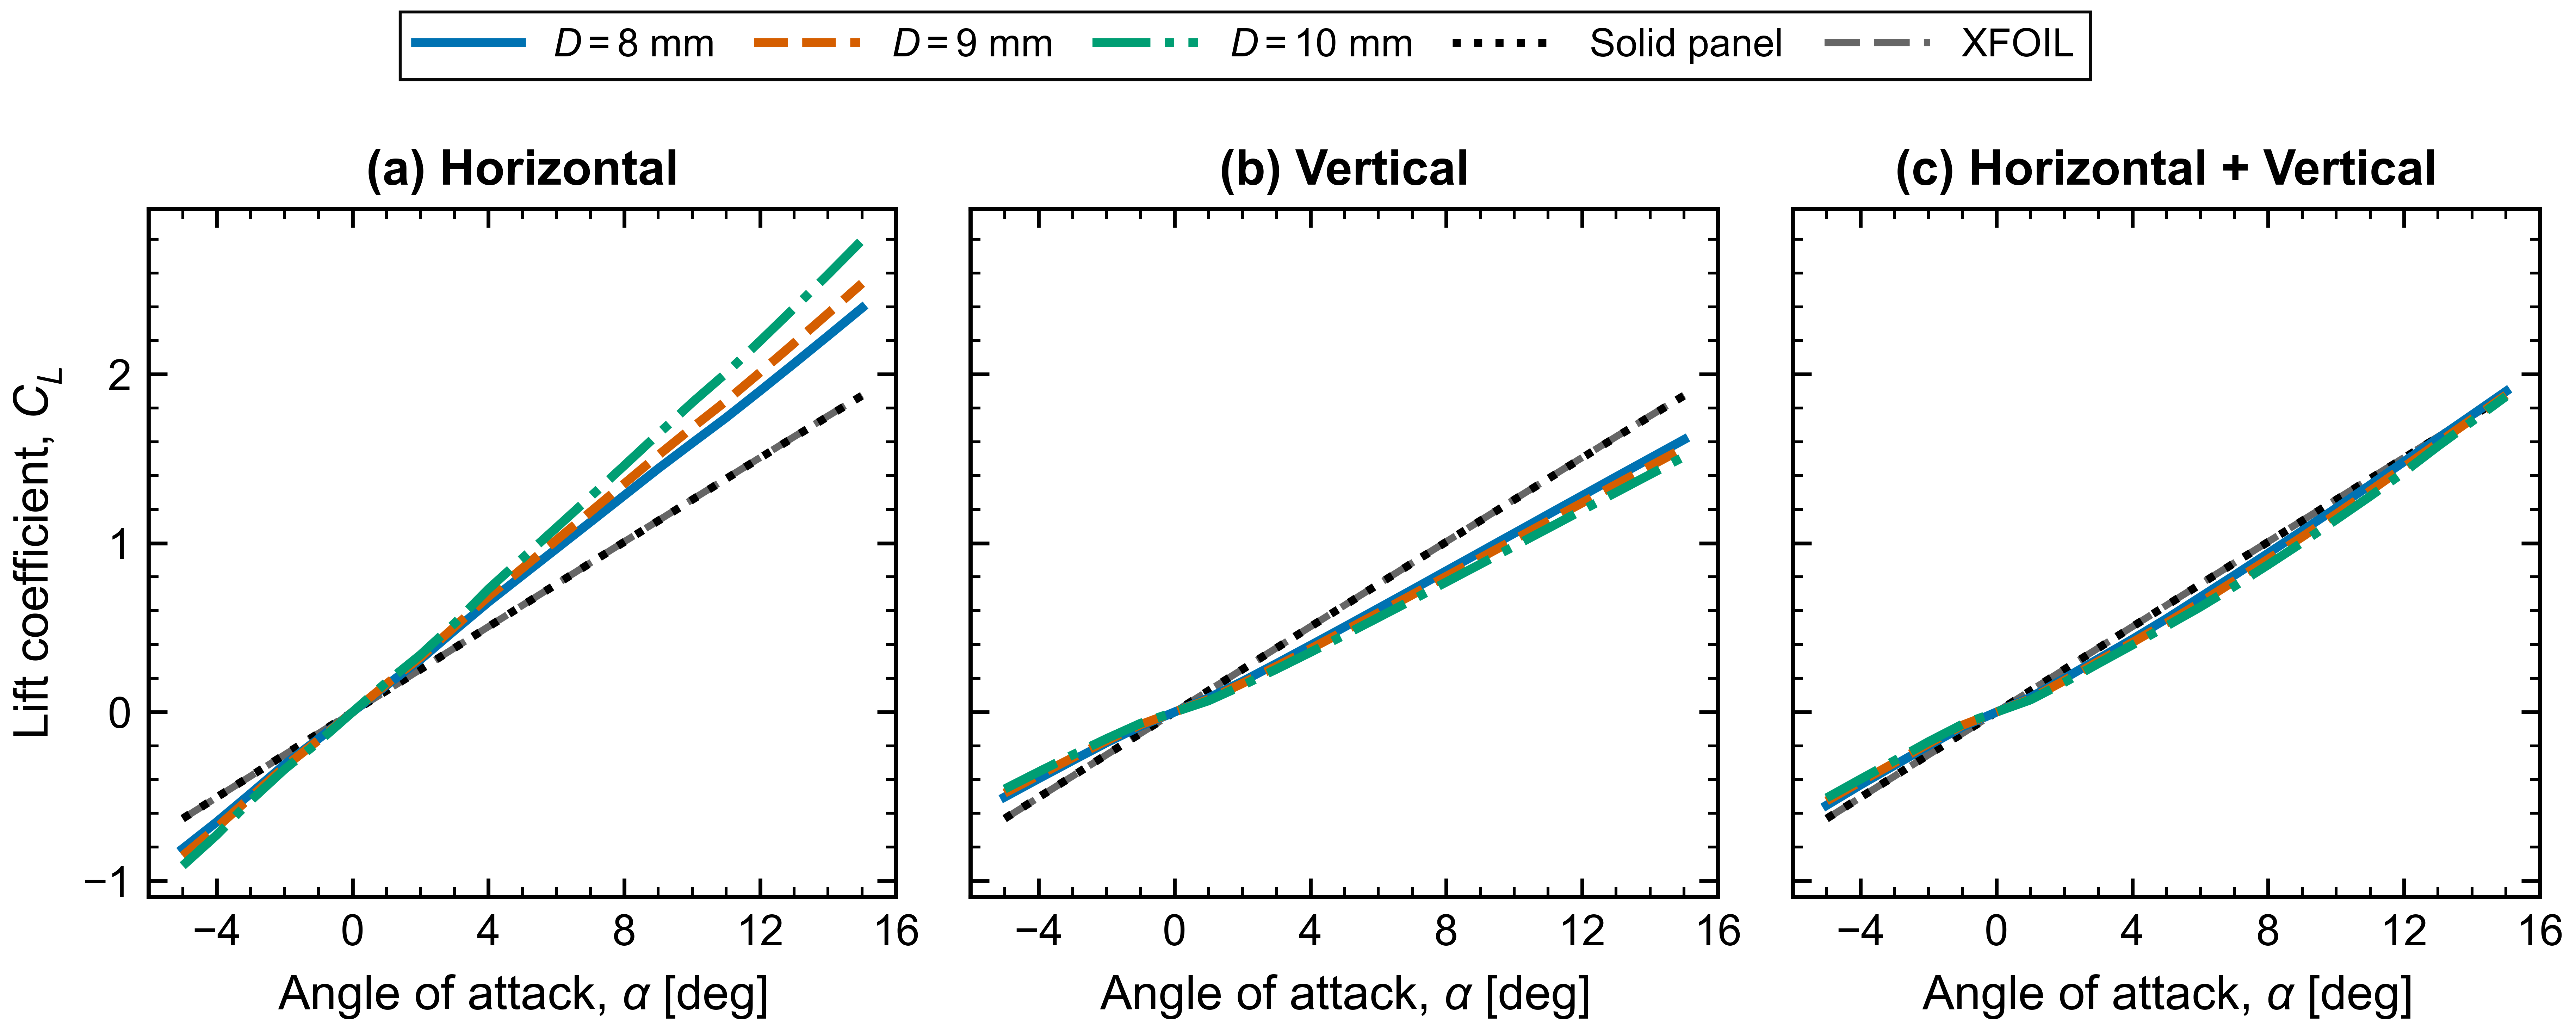
\includegraphics[
	width=0.96\textwidth
	]{figs/CL_vs_AoA_three_models_three_diameters.png}
	\caption{
		Lift coefficient as a function of angle of attack for
		(a) the horizontal model (M1),
		(b) the vertical model (M2), and
		(c) the combined horizontal--vertical model (M3).
		Results are shown for circular-channel diameters
		$D=8$, $9$ and $10~\mathrm{mm}$ together with the
		impermeable panel-method and XFOIL reference solutions.
	}
	\label{fig:cl_aoa_three_models}
\end{figure*}

The horizontal configuration produces the largest modification of the
lift response. At positive angles of attack, the porous horizontal
cases develop a larger lift coefficient than the impermeable reference,
and the difference increases progressively with angle of attack.
Increasing the channel diameter further strengthens this effect, with
the $D=10~\mathrm{mm}$ configuration producing the largest lift
coefficient over the upper part of the investigated angle-of-attack
range.

The same diameter dependence is also apparent at negative angles of
attack, where increasing the channel diameter increases the magnitude
of the negative lift. The approximately antisymmetric response about
the zero-lift region is consistent with the symmetric NACA~0018
geometry and indicates that the horizontal channels primarily modify
the aerodynamic loading generated as the angle of attack departs from
zero.

The vertical configuration exhibits a distinctly different response.
At positive angles of attack, the lift coefficient is generally lower
than that of the impermeable airfoil. Furthermore, the three channel
diameters remain relatively close to one another throughout most of
the sweep. The aerodynamic influence of the vertical configuration is
therefore less sensitive to channel diameter than that of the
horizontal arrangement.

For the combined horizontal--vertical configuration, the porous
solutions remain relatively close to the impermeable reference over a
large part of the angle-of-attack range. At positive angles of attack,
the lift coefficient is generally slightly lower than the solid-airfoil
solution before approaching the reference towards the upper end of the
sweep. The three channel diameters also remain closely grouped.

These results demonstrate that the aerodynamic effect of porosity
depends strongly on the orientation of the internal channels rather
than on channel diameter alone. In particular, increasing diameter
does not produce a universal increase in lift. A strong diameter effect
is observed for M1, whereas M2 and M3 show considerably weaker
sensitivity. This indicates that the pressure difference established
between the connected surface locations is a critical factor governing
the resulting internal flow and aerodynamic response.


% ============================================================
% PITCHING MOMENT
% ============================================================

\subsection{Effect of porous-channel configuration on pitching moment}
\label{subsec:moment_results}

The corresponding quarter-chord pitching-moment coefficients are
presented in Fig.~\ref{fig:cm_aoa_three_models}.

\begin{figure*}
	\centering
	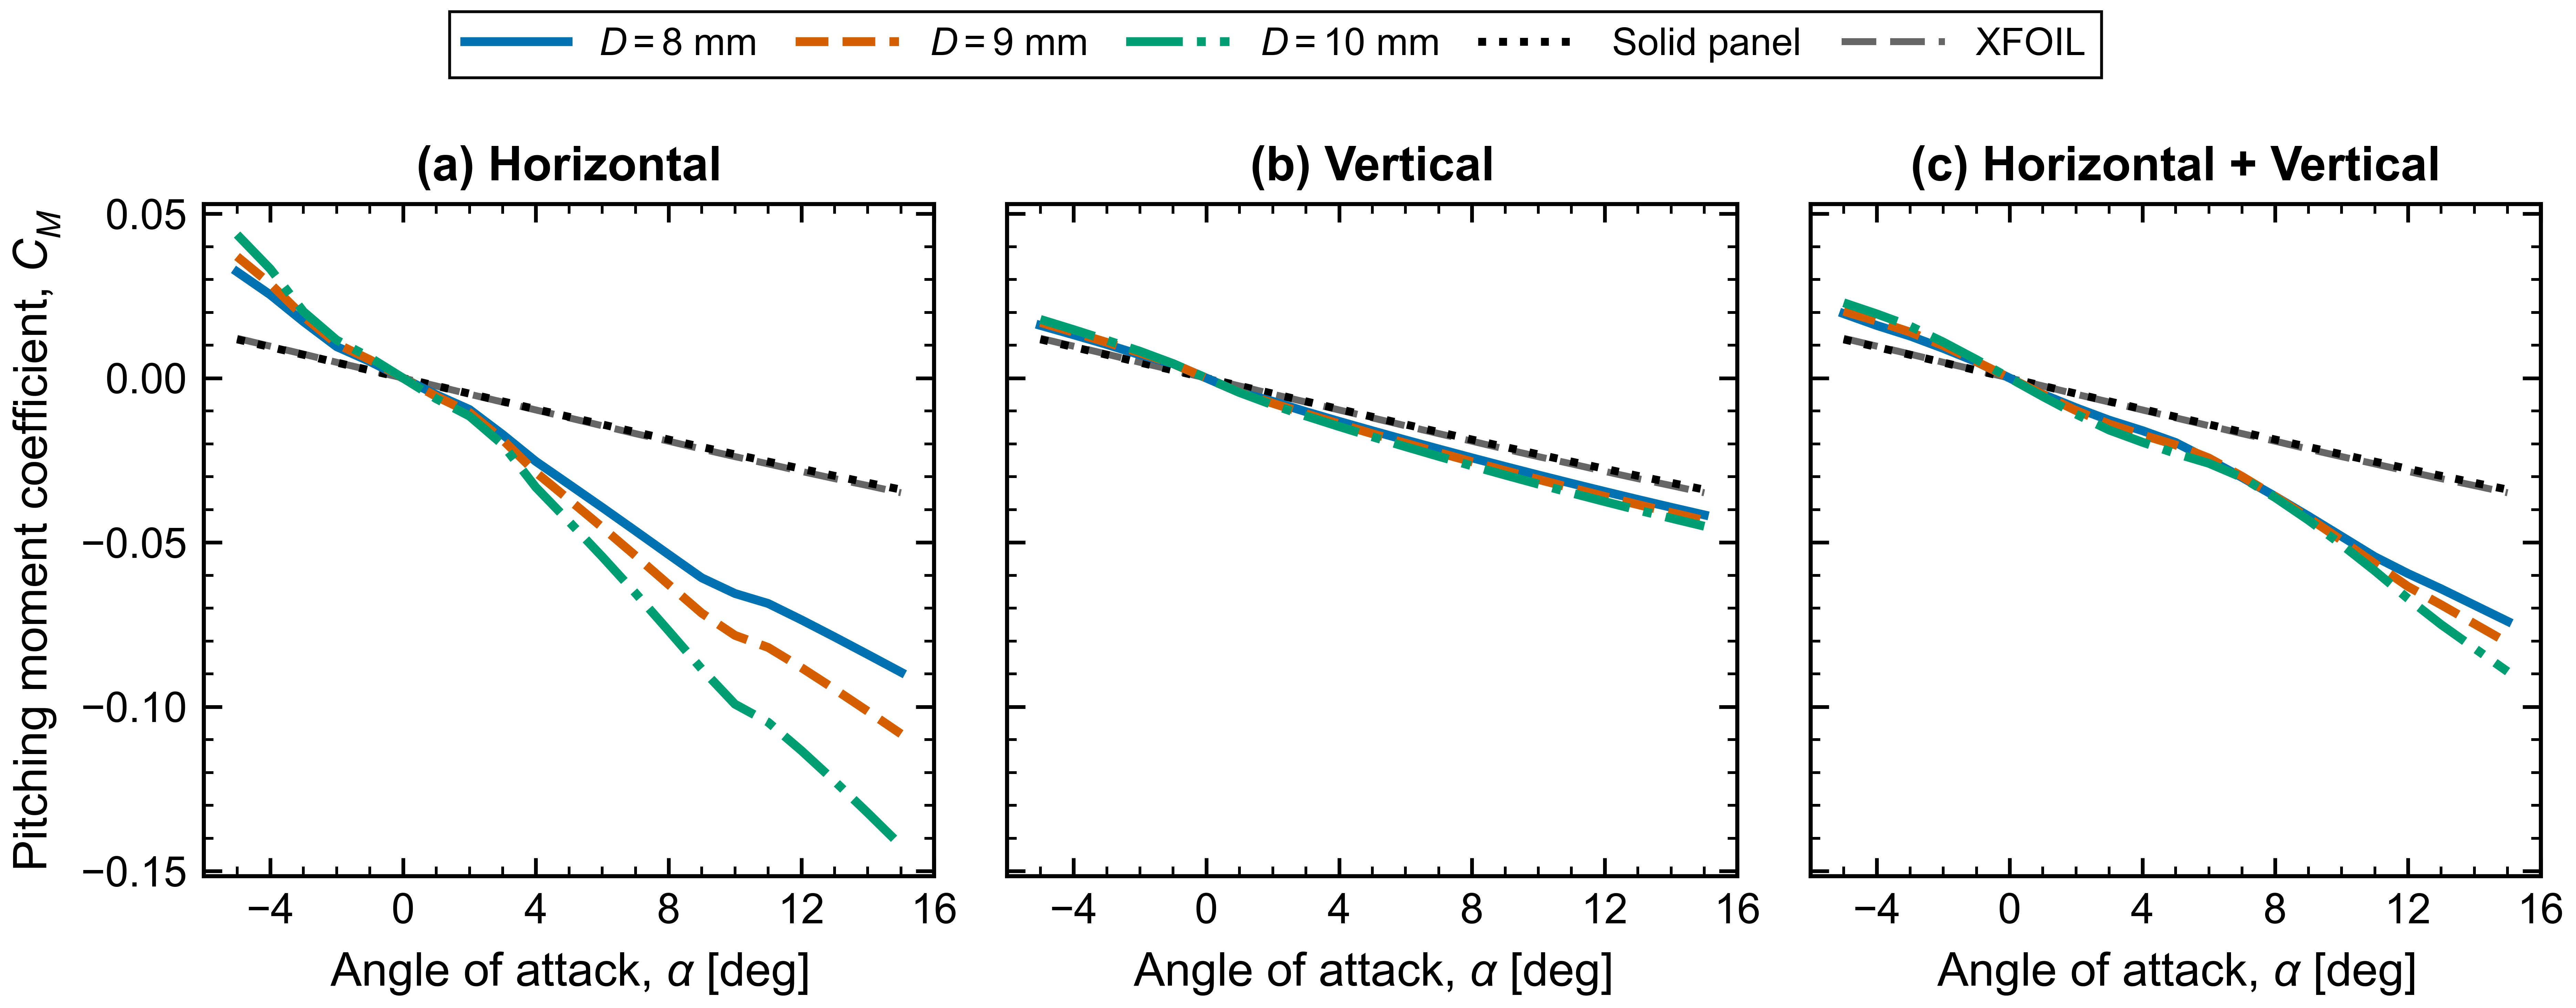
\includegraphics[
	width=0.96\textwidth
	]{figs/CM_vs_AoA_three_models_three_diameters.png}
	\caption{
		Pitching-moment coefficient about the quarter chord as a
		function of angle of attack for
		(a) the horizontal model (M1),
		(b) the vertical model (M2), and
		(c) the combined horizontal--vertical model (M3).
		Results are shown for circular-channel diameters
		$D=8$, $9$ and $10~\mathrm{mm}$ together with the
		impermeable panel-method and XFOIL reference solutions.
	}
	\label{fig:cm_aoa_three_models}
\end{figure*}

The horizontal configuration again produces the strongest departure
from the impermeable-airfoil behaviour. As the angle of attack
increases, the porous cases develop an increasingly negative pitching
moment relative to the solid reference. The magnitude of this change
also increases with channel diameter, with the $D=10~\mathrm{mm}$
case showing the largest negative pitching moment at high positive
angles of attack.

The increase in lift produced by M1 is therefore accompanied by a
corresponding modification of the pitching moment. This represents an
important aerodynamic trade-off: the configuration that produces the
largest lift enhancement also causes the largest change in the
longitudinal aerodynamic loading.

The vertical configuration produces substantially smaller changes in
pitching moment. The three channel diameters remain closely grouped
throughout the angle-of-attack sweep, consistent with the relatively
weak diameter sensitivity observed in the corresponding lift results.
At positive angles of attack, the porous configurations become
slightly more negative than the impermeable reference as the angle of
attack increases.

The combined configuration shows behaviour between that of the
horizontal and vertical arrangements. The pitching moment becomes more
negative at increasing positive angle of attack, although the departure
from the impermeable solution remains smaller than that obtained for
the horizontal configuration. Diameter sensitivity also becomes more
visible towards the upper end of the angle-of-attack range.

The lift and pitching-moment results therefore show that channel
orientation affects not only the magnitude of the aerodynamic force
but also its distribution along the chord. The particularly strong
changes observed for M1 suggest that the horizontal passages cause a
larger redistribution of surface pressure than the vertical passages.


% ============================================================
% FLOW FIELD
% ============================================================

\subsection{Flow-field modification induced by the porous channels}
\label{subsec:flowfield_results}

To examine the origin of the changes observed in the integrated
aerodynamic coefficients, the porous-airfoil pressure and velocity
fields are compared with the corresponding impermeable-airfoil
solution. The comparison is performed at

\begin{equation}
	\alpha=10^\circ,
	\qquad
	D=9~\mathrm{mm}.
\end{equation}

This condition provides a representative positive angle of attack at
which the aerodynamic effect of the porous channels is clearly
developed.


\subsubsection{Pressure-field modification}

Figure~\ref{fig:pressure_difference} shows the pressure difference

\begin{equation}
	\Delta p_{\mathrm{field}}
	=
	p_{\mathrm{porous}}
	-
	p_{\mathrm{solid}},
	\label{eq:pressure_field_difference}
\end{equation}

for the three porous configurations.

\begin{figure*}
	\centering
	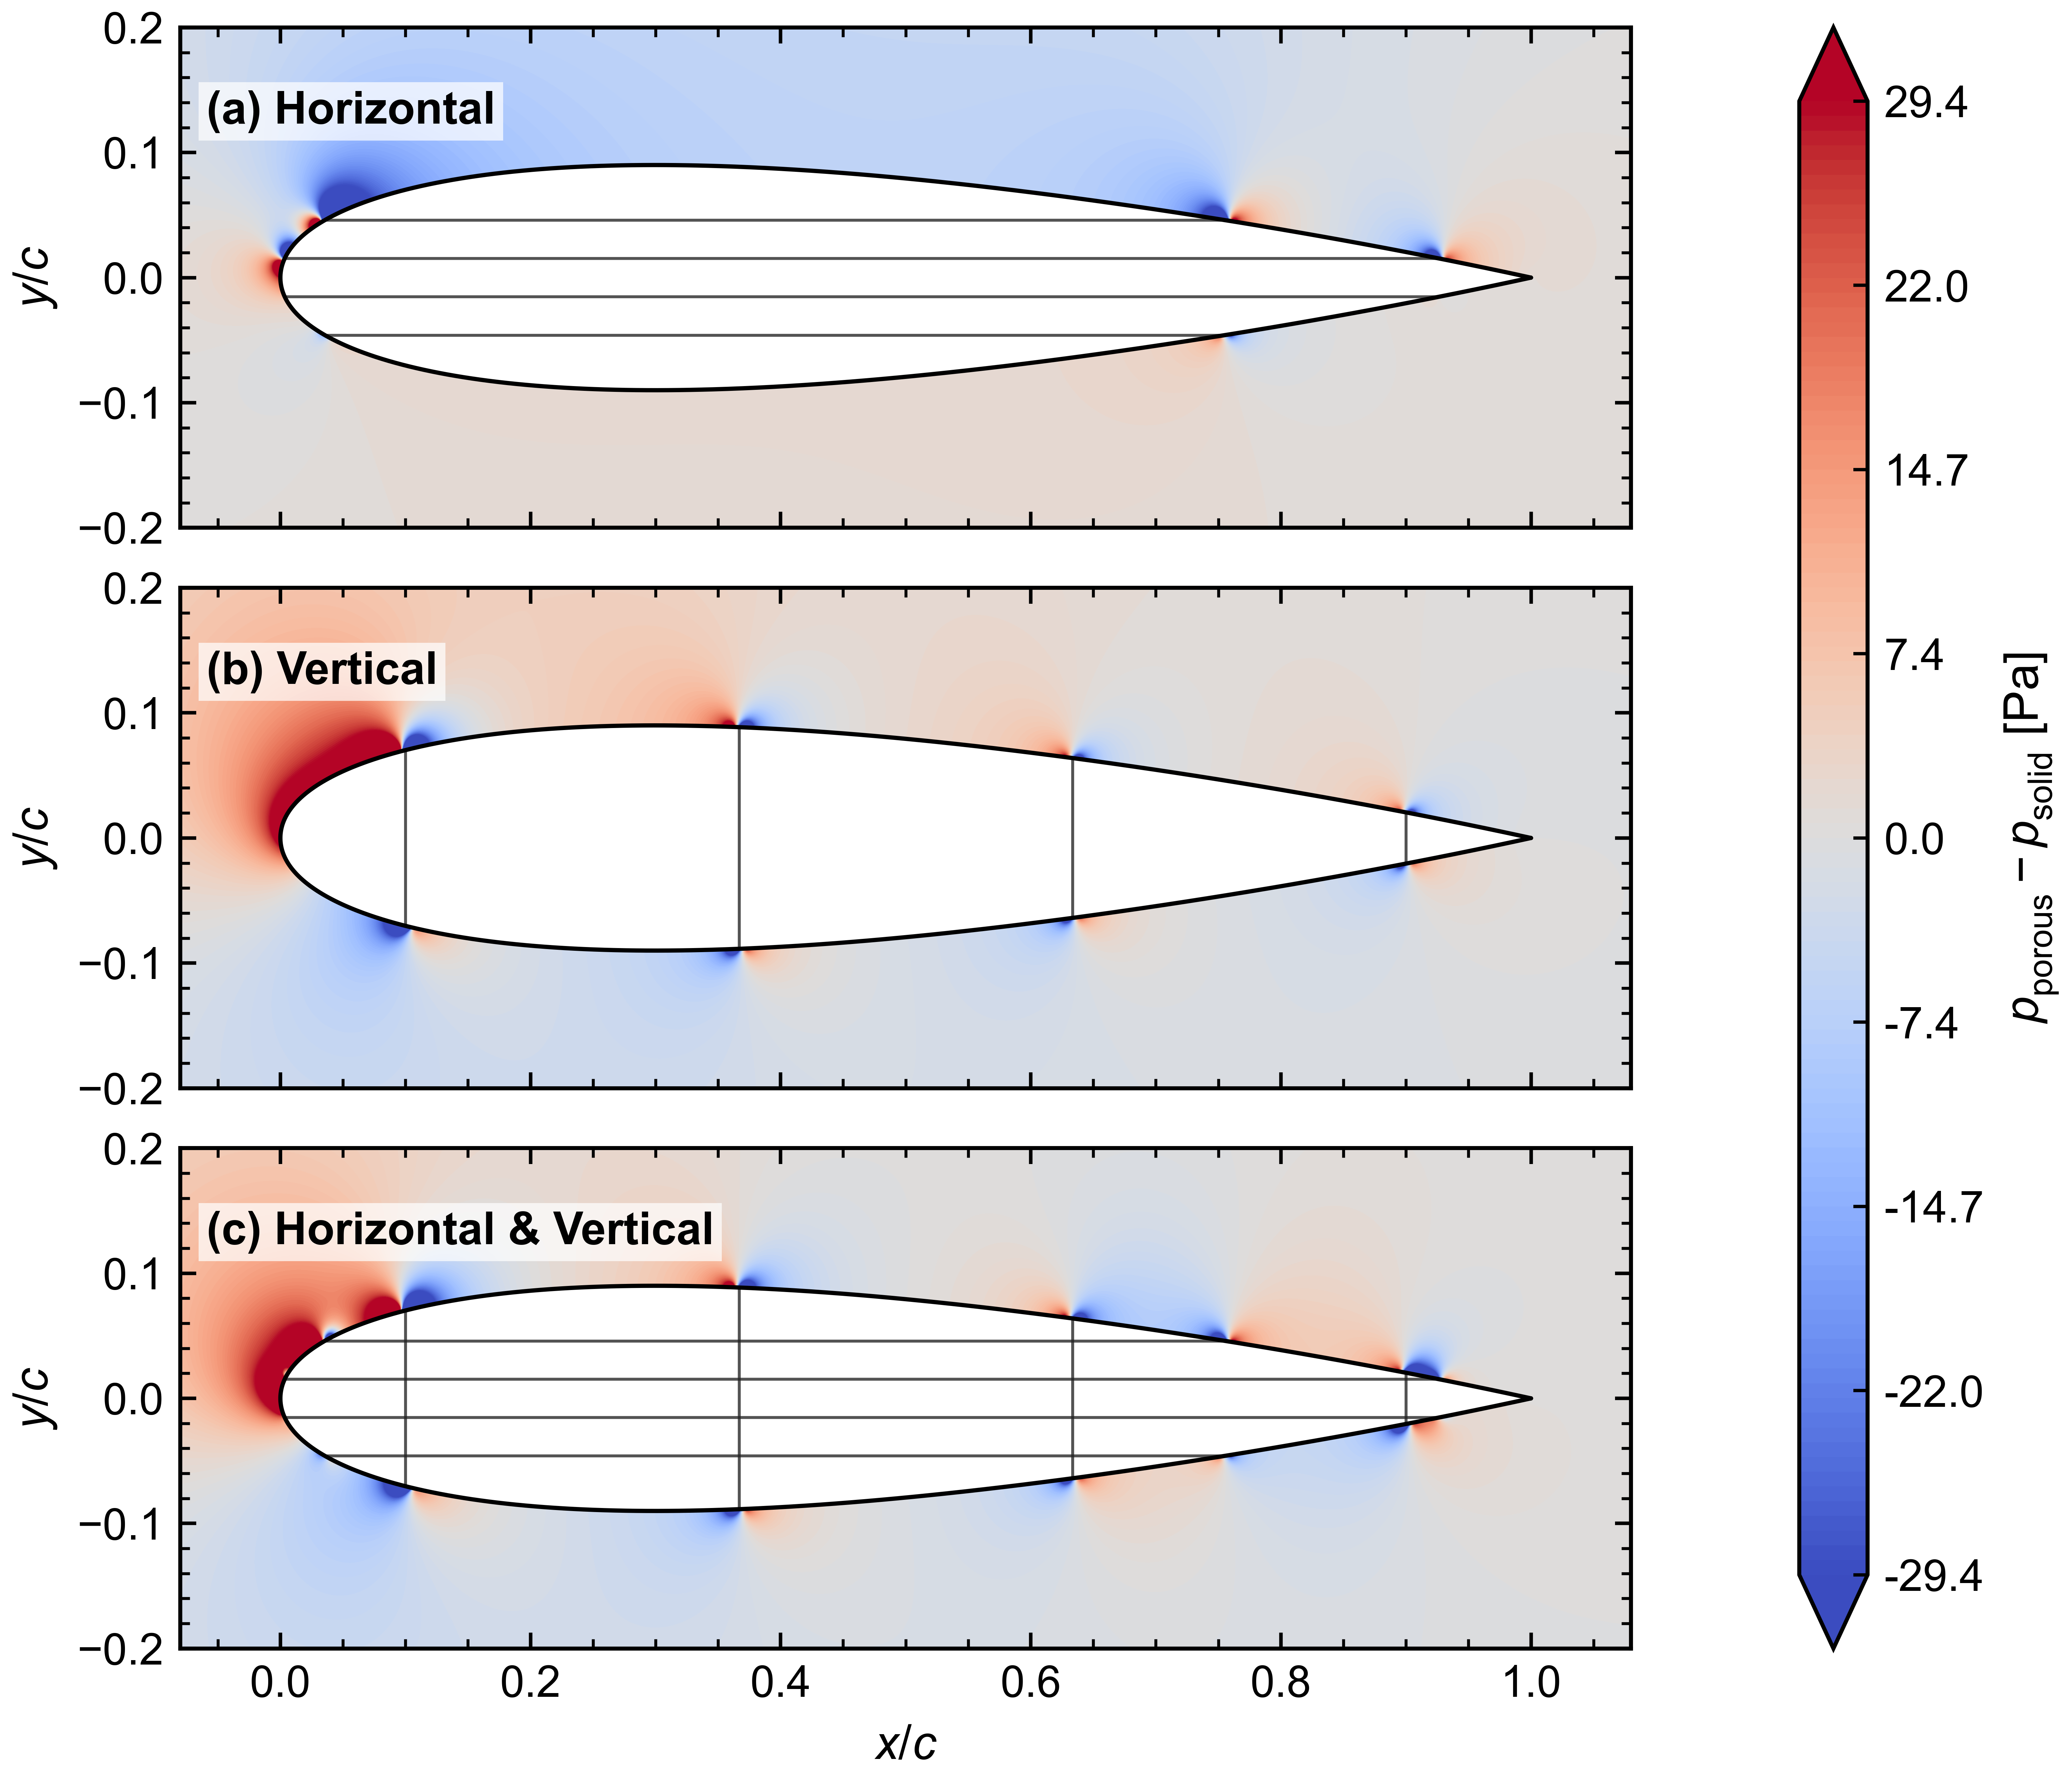
\includegraphics[
	width=0.62\textwidth
	]{figs/pressure_difference_pa_portrait_one_colorbar.png}
	\caption{
		Pressure-field difference between the porous and
		impermeable airfoils at $\alpha=10^\circ$ and
		$D=9~\mathrm{mm}$ for
		(a) the horizontal model (M1),
		(b) the vertical model (M2), and
		(c) the combined horizontal--vertical model (M3).
		Positive values represent an increase in pressure relative
		to the impermeable airfoil and negative values represent a
		reduction.
	}
	\label{fig:pressure_difference}
\end{figure*}

The pressure changes are concentrated primarily around the channel
openings, confirming that the imposed transpiration modifies the local
external pressure field. Adjacent regions of positive and negative
pressure difference occur around several openings, indicating local
redistribution of the aerodynamic loading rather than a uniform
pressure shift over the complete surface.

For the horizontal configuration, the pressure differences are
predominantly localised around the individual chordwise openings.
Distinct pressure increases and reductions are generated on both the
upper and lower surfaces. Although these regions remain spatially
localised, their cumulative influence modifies the integrated surface
loading sufficiently to produce the substantial increase in lift and
pitching-moment magnitude observed in
Figs.~\ref{fig:cl_aoa_three_models} and
\ref{fig:cm_aoa_three_models}.

The vertical configuration produces a different spatial pattern.
In addition to the local pressure changes at individual openings, a
comparatively broad pressure modification develops around the
leading-edge region. Since each vertical passage connects the lower
and upper surfaces, the pressure-driven internal flow directly couples
regions subjected to different external aerodynamic loading.

The combined configuration contains features associated with both the
horizontal and vertical arrangements. Localised pressure changes are
observed at the horizontal-channel openings, while the vertical
passages introduce additional upper-to-lower surface interaction.
However, the resulting integrated lift response does not equal the
strong enhancement obtained for the horizontal model alone. This
demonstrates that superposing the two channel arrangements does not
produce a simple additive aerodynamic effect.


\subsubsection{Velocity-field modification}

The corresponding difference in external velocity magnitude is shown
in Fig.~\ref{fig:velocity_difference}. The plotted quantity is

\begin{equation}
	\Delta |\boldsymbol{V}|
	=
	|\boldsymbol{V}|_{\mathrm{porous}}
	-
	|\boldsymbol{V}|_{\mathrm{solid}}.
	\label{eq:velocity_field_difference}
\end{equation}

\begin{figure*}
	\centering
	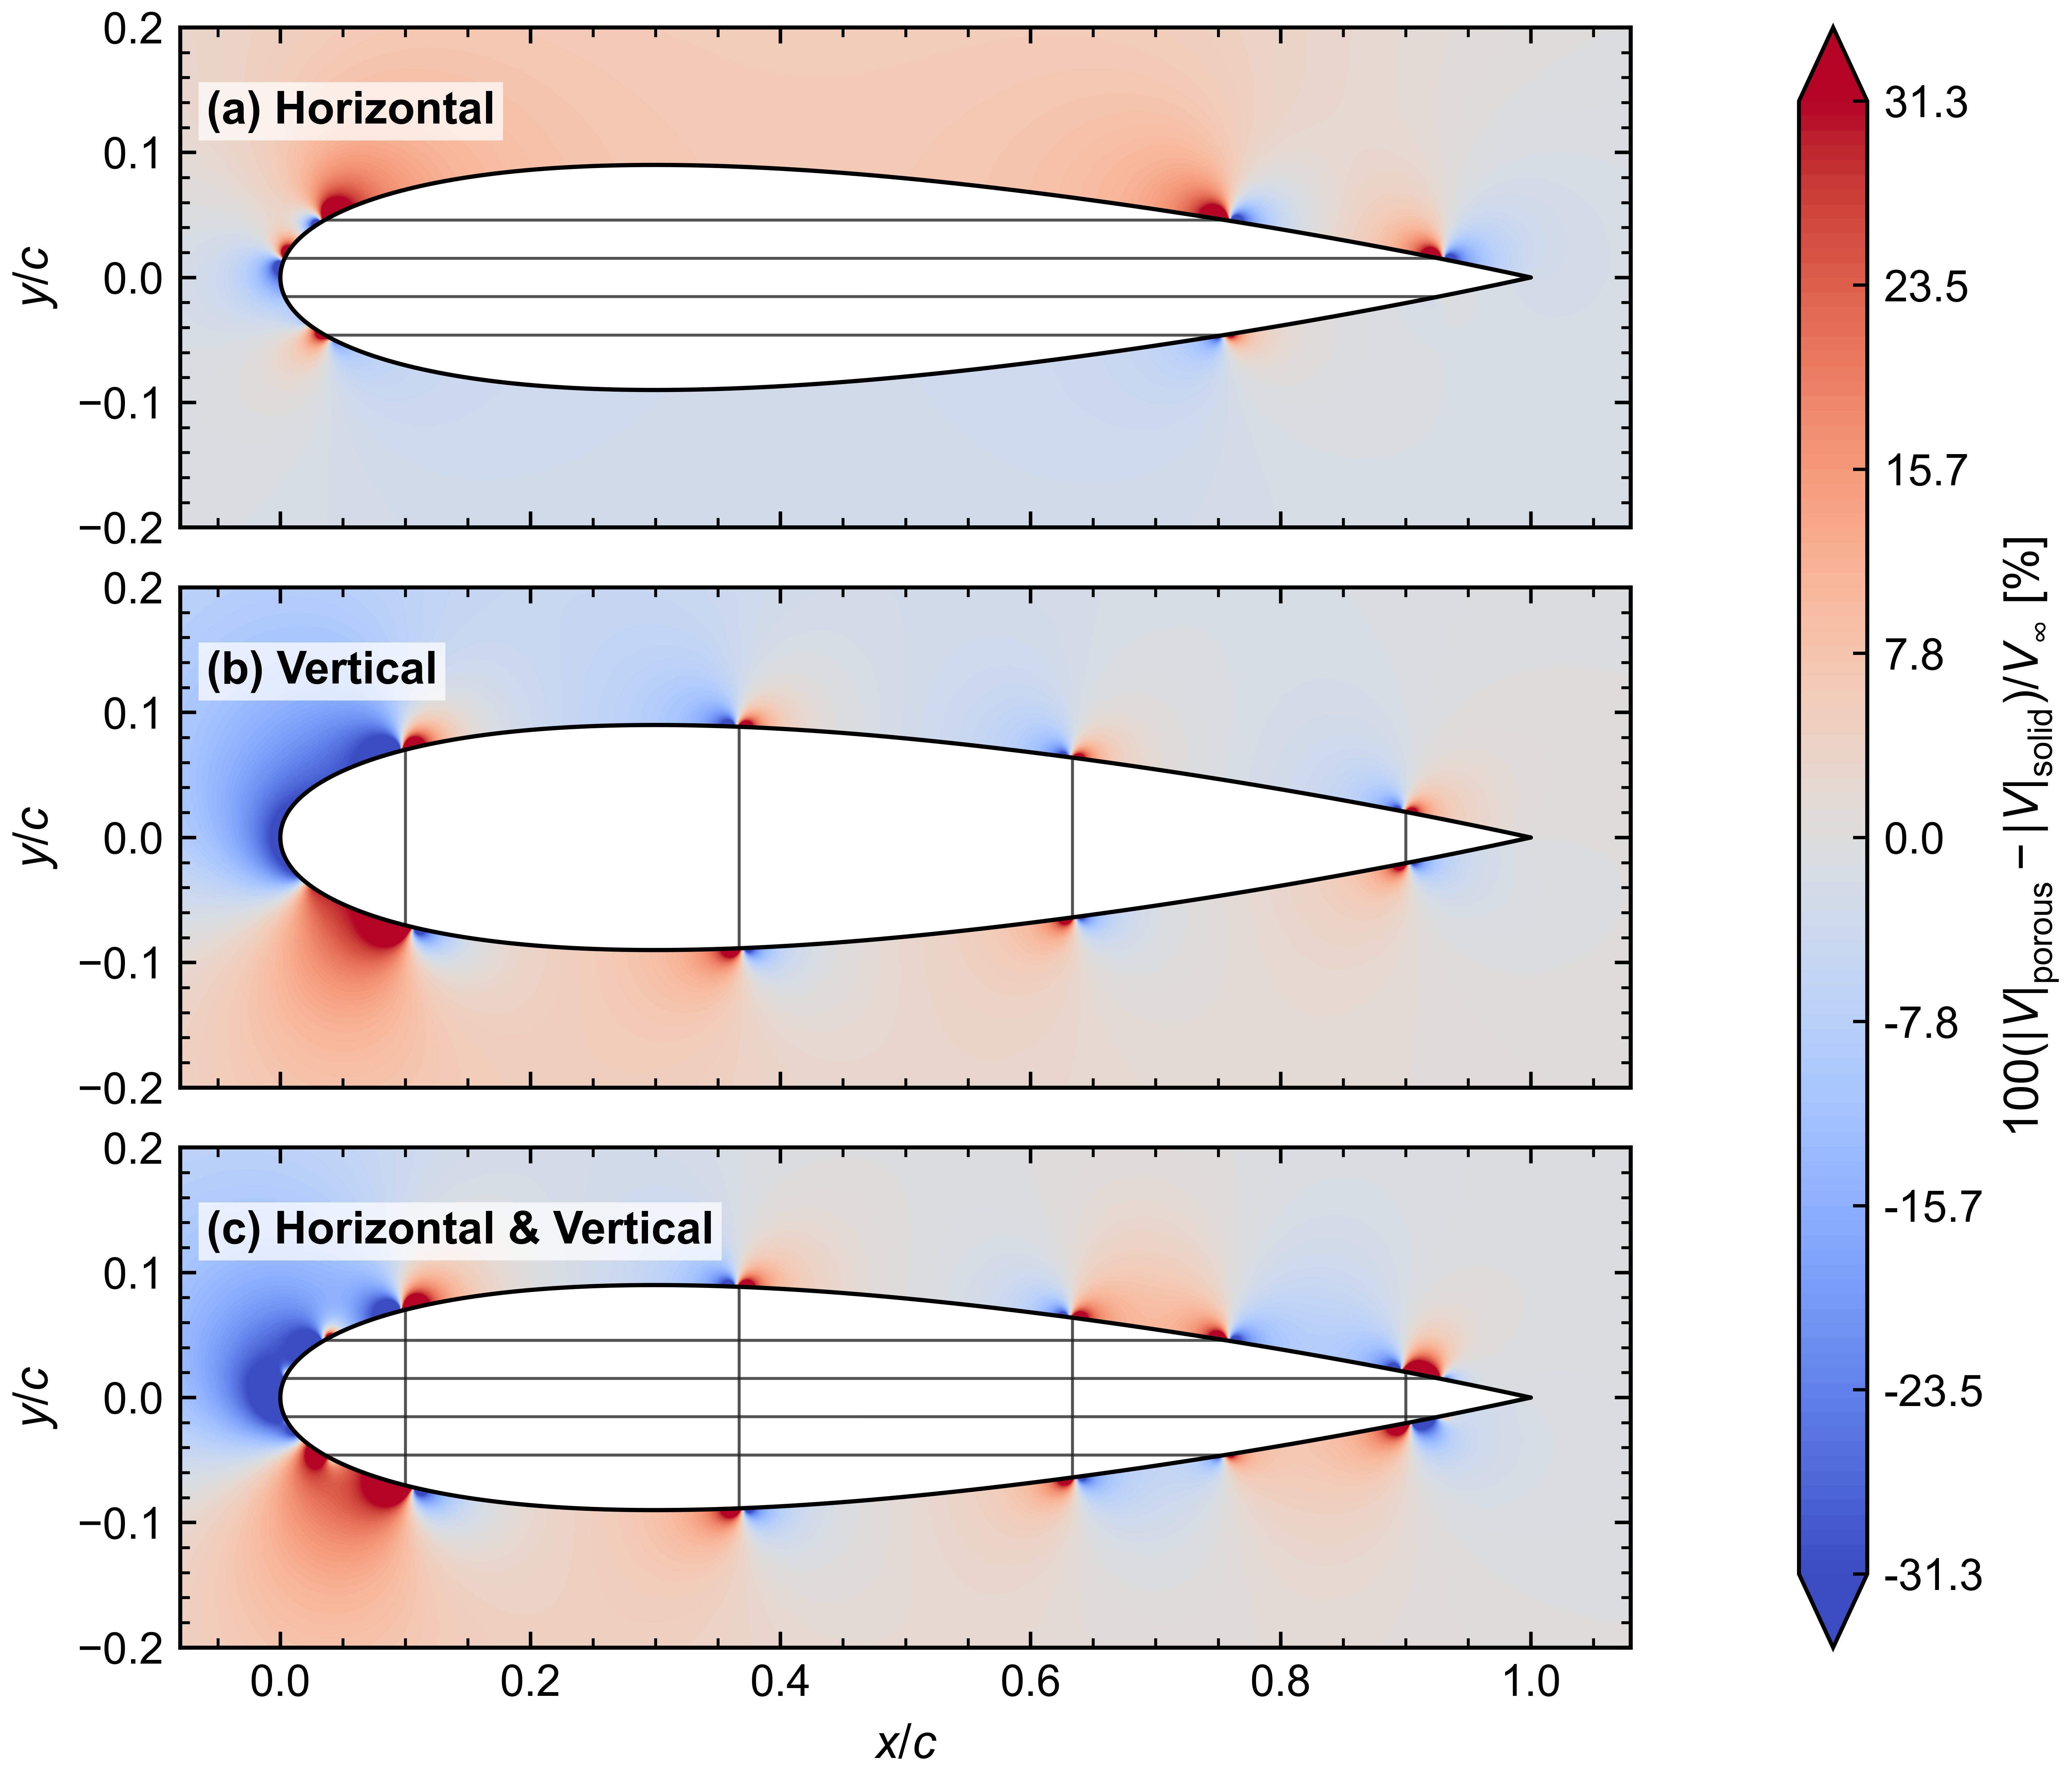
\includegraphics[
	width=0.62\textwidth
	]{figs/velocity_difference_percent_portrait_one_colorbar.png}
	\caption{
		Difference in velocity magnitude between the porous and
		impermeable-airfoil solutions at $\alpha=10^\circ$ and
		$D=9~\mathrm{mm}$ for
		(a) the horizontal model (M1),
		(b) the vertical model (M2), and
		(c) the combined horizontal--vertical model (M3).
		Positive values indicate an increase in velocity magnitude
		and negative values indicate a reduction relative to the
		impermeable solution.
	}
	\label{fig:velocity_difference}
\end{figure*}

The velocity-field differences show a spatial distribution consistent
with the pressure-field modifications. The strongest changes occur
close to the channel openings, where the surface-normal transpiration
directly alters the local external flow.

The horizontal configuration produces alternating regions of
acceleration and deceleration around the chordwise openings. The
modifications remain concentrated close to the airfoil surface,
although their influence extends into the surrounding external flow.
These local changes alter the surface velocity and therefore the
pressure coefficient through the Bernoulli relation.

For the vertical configuration, a broader velocity modification is
visible around the leading-edge region together with local changes at
the remaining channel openings. This behaviour corresponds closely to
the pressure redistribution observed in
Fig.~\ref{fig:pressure_difference}. The resulting modification of the
upper- and lower-surface velocities reduces the lift relative to the
impermeable case over much of the positive angle-of-attack range.

The combined configuration again exhibits characteristics of both M1
and M2. Velocity changes are present around both the horizontal and
vertical opening locations, but their interaction produces a different
overall aerodynamic response from either individual configuration.


% ============================================================
% OVERALL COMPARISON
% ============================================================

\subsection{Overall comparison of porous configurations}
\label{subsec:overall_comparison}

The combined aerodynamic and flow-field results demonstrate that the
orientation of the internal channels is the dominant parameter
governing the effect of the passive porous system.

Among the configurations investigated, the horizontal model produces
the strongest modification of the aerodynamic response. At positive
angles of attack, M1 increases the lift coefficient relative to the
impermeable reference, with the magnitude of the enhancement increasing
with channel diameter. However, this lift enhancement is accompanied by
a progressively more negative pitching moment, particularly for the
larger channel diameters.

The vertical configuration produces a comparatively weaker dependence
on channel diameter and generally reduces the lift coefficient relative
to the impermeable airfoil at positive angles of attack. Its effect on
pitching moment is also considerably smaller than that of the
horizontal configuration.

The combined horizontal--vertical configuration does not simply
superpose the aerodynamic behaviour of M1 and M2. Despite containing
the horizontal passages responsible for the strongest lift enhancement
in M1, the additional vertical passages alter the pressure and velocity
redistribution such that the overall lift response remains much closer
to the impermeable-airfoil solution.

The pressure- and velocity-difference fields support these integrated
aerodynamic trends. The strongest local modifications occur around the
channel openings, while the orientation and connectivity of the
passages determine how these local changes are distributed between the
upper and lower airfoil surfaces. Consequently, the aerodynamic
performance of the porous airfoil depends not only on channel size but
also strongly on the placement and orientation of the internal flow
paths.

Overall, the horizontal configuration provides the greatest potential
for increasing lift among the three configurations investigated.
However, the accompanying pitching-moment change indicates that the
selection of a porous-channel arrangement should consider the combined
effect on aerodynamic force and moment rather than lift enhancement
alone.
\section{Installation}

The package is available at author resources page at Elsevier
(\url{http://www.elsevier.com/locate/latex}).
The class may be moved or copied to a place, usually,\linebreak
\verb+$TEXMF/tex/latex/elsevier/+, %$%%%%%%%%%%%%%%%%%%%%%%%%%%%%
or a folder which will be read                   
by \LaTeX{} during document compilation.  The \TeX{} file
database needs updation after moving/copying class file.  Usually,
we use commands like \verb+mktexlsr+ or \verb+texhash+ depending
upon the distribution and operating system.

\section{Front matter}

The author names and affiliations could be formatted in two ways:
\begin{enumerate}[(1)]
	\item Group the authors per affiliation.
	\item Use footnotes to indicate the affiliations.
\end{enumerate}
See the front matter of this document for examples. 
You are recommended to conform your choice to the journal you 
are submitting to.

\section{Bibliography styles}

There are various bibliography styles available. You can select the
style of your choice in the preamble of this document. These styles are
Elsevier styles based on standard styles like Harvard and Vancouver.
Please use Bib\TeX\ to generate your bibliography and include DOIs
whenever available.

Here are two sample references: 
\cite{Fortunato2010}
\cite{Fortunato2010,NewmanGirvan2004}
\cite{Fortunato2010,Vehlowetal2013}

\section{Floats}
{Figures} may be included using the command,\linebreak 
\verb+\includegraphics+ in
combination with or without its several options to further control
graphic. \verb+\includegraphics+ is provided by {graphic[s,x].sty}
which is part of any standard \LaTeX{} distribution.
{graphicx.sty} is loaded by default. \LaTeX{} accepts figures in
the postscript format while pdf\LaTeX{} accepts {*.pdf},
{*.mps} (metapost), {*.jpg} and {*.png} formats. 
pdf\LaTeX{} does not accept graphic files in the postscript format. 

\begin{figure}
	\centering
	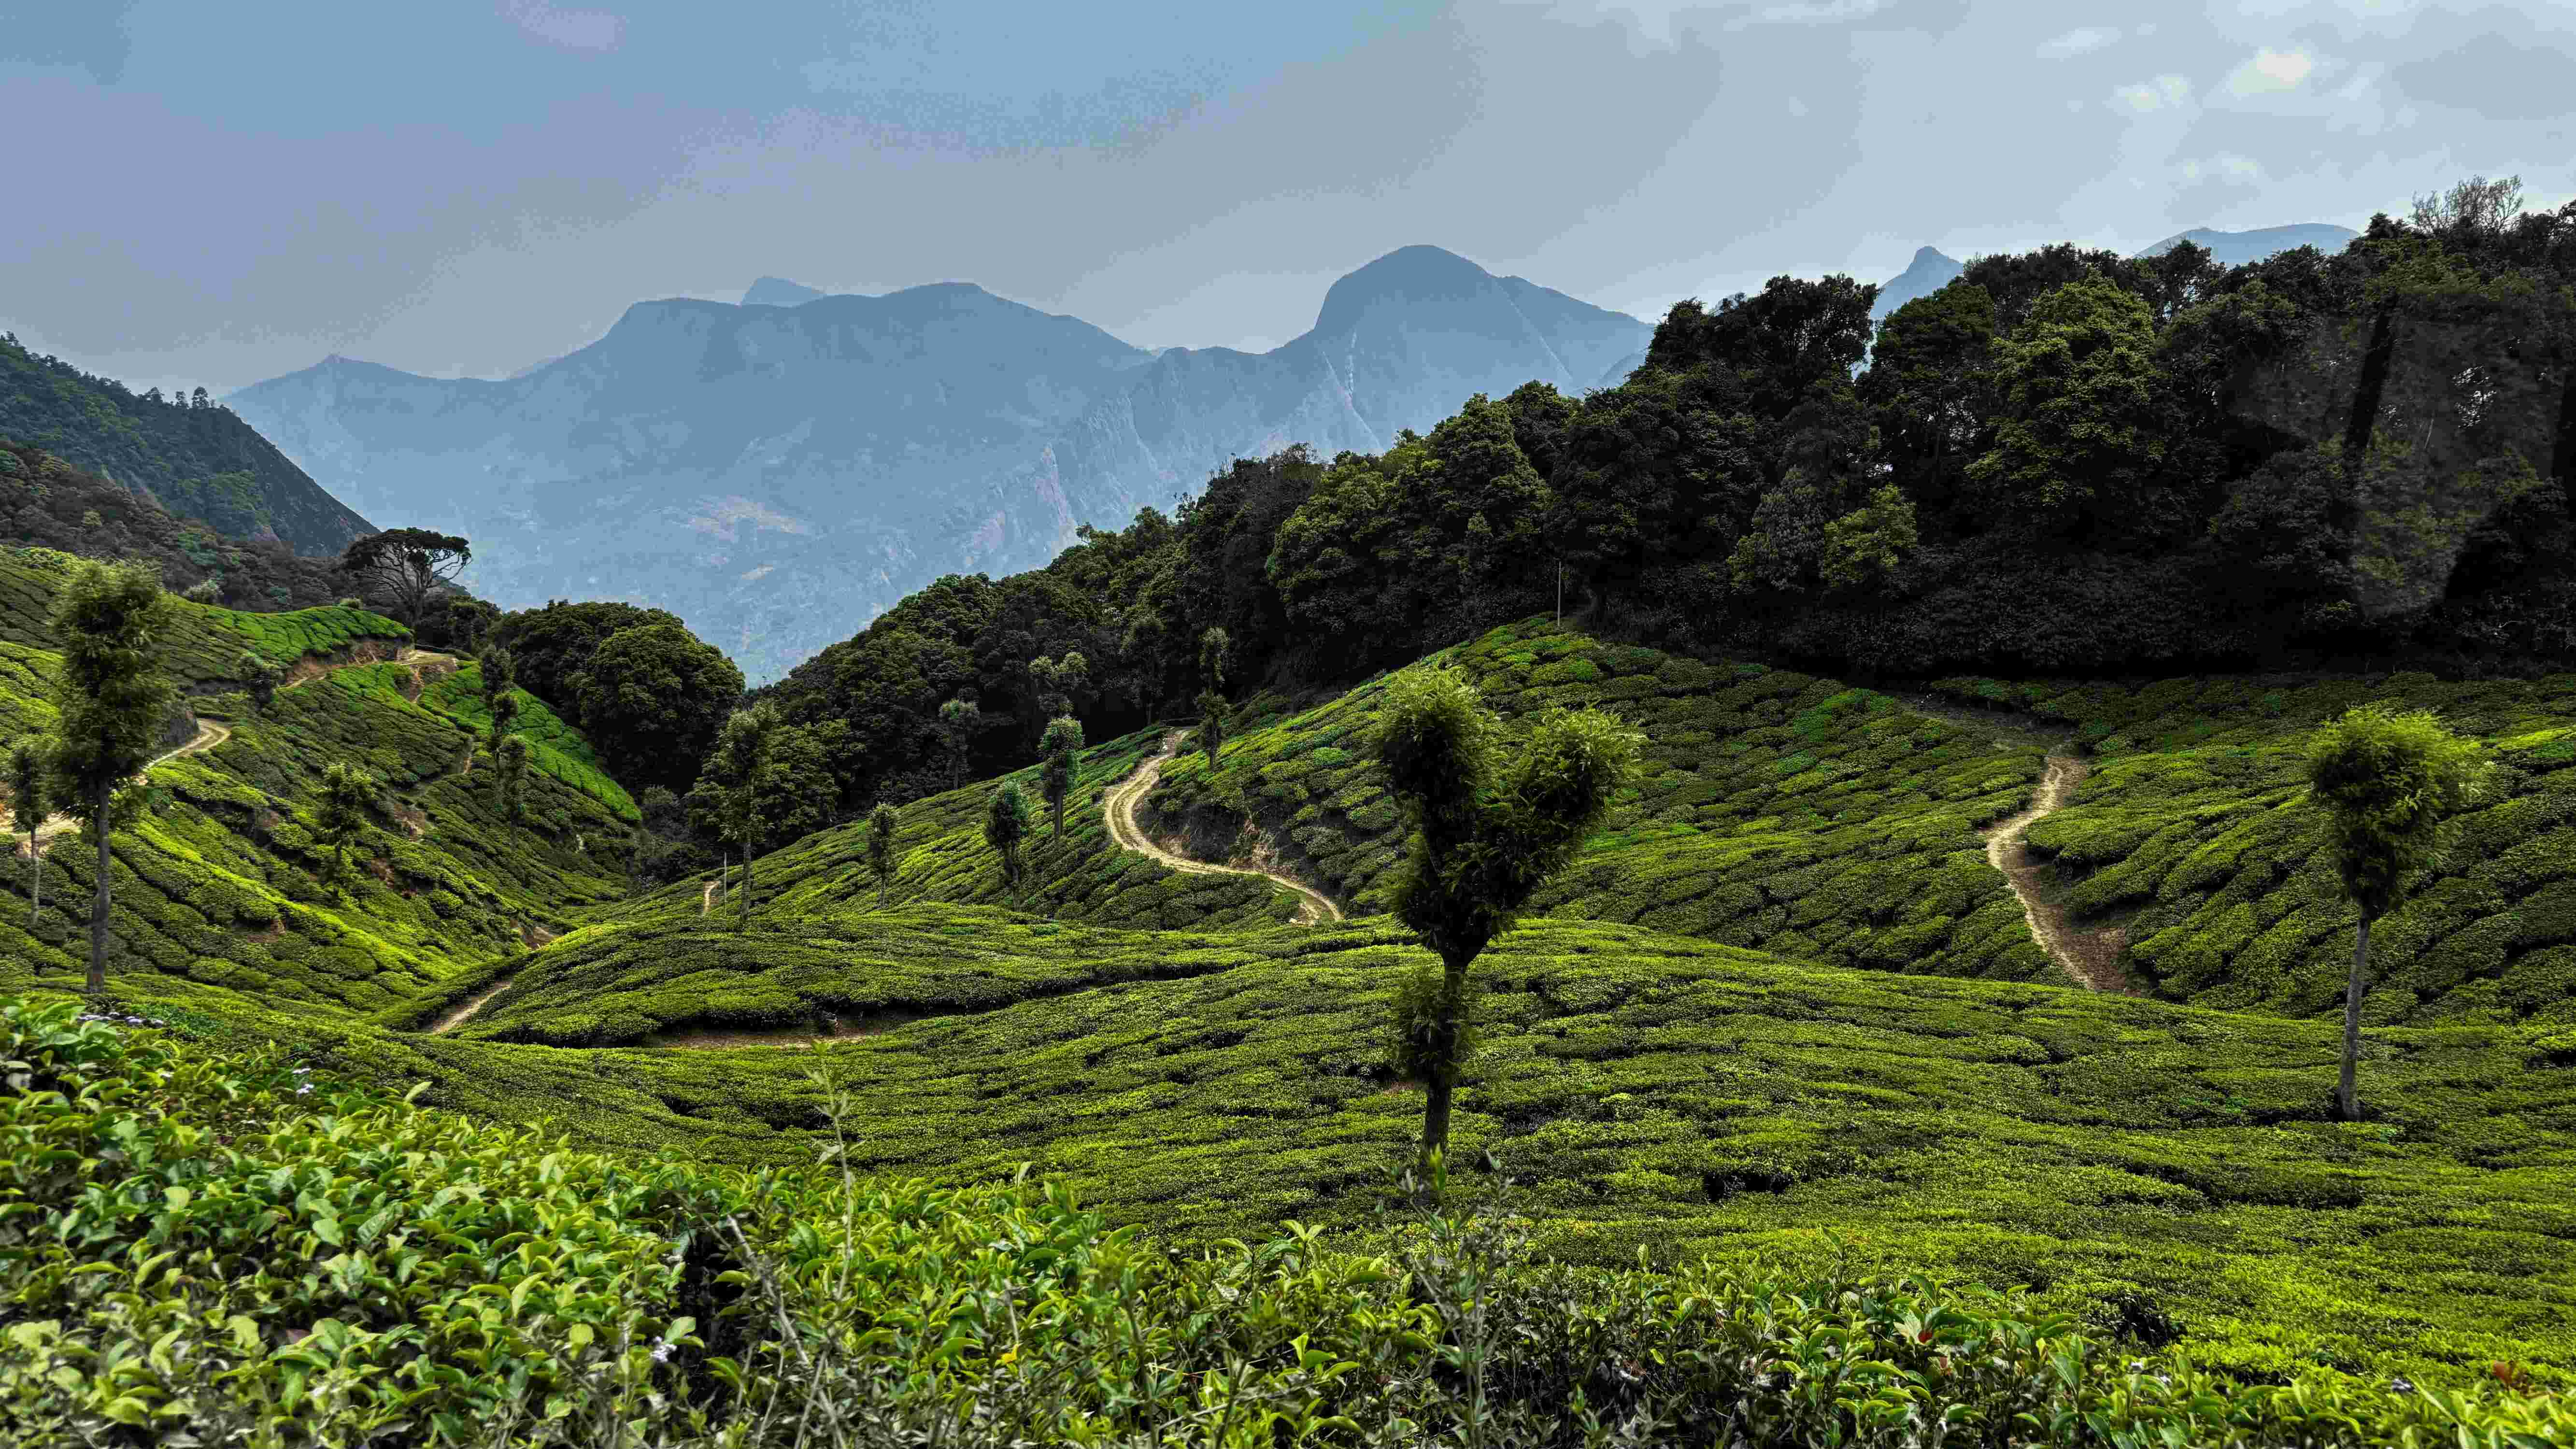
\includegraphics[width=.9\columnwidth]{figs/cas-munnar-2024.jpg}
	\caption{The beauty of Munnar, Kerala. (See also Table \protect\ref{tbl1}).}
	\label{FIG:1}
\end{figure}


The \verb+table+ environment is handy for marking up tabular
material. If users want to use {multirow.sty},
{array.sty}, etc., to fine control/enhance the tables, they
are welcome to load any package of their choice and
{cas-dc.cls} will work in combination with all loaded
packages.

\begin{table}[width=.9\linewidth,cols=4,pos=h]
	\caption{This is a test caption. This is a test caption. This is a test
		caption. This is a test caption. Use \{table*\} instead of \{table\} if you
		want a two column spanned table.}\label{tbl1}
	\begin{tabular*}{\tblwidth}{@{} LLLL@{} }
		\toprule
		Col 1 & Col 2 & Col 3 & Col4\\
		\midrule
		12345 & 12345 & 123 & 12345 \\
		12345 & 12345 & 123 & 12345 \\
		12345 & 12345 & 123 & 12345 \\
		12345 & 12345 & 123 & 12345 \\
		12345 & 12345 & 123 & 12345 \\
		\bottomrule
	\end{tabular*}
\end{table}

\section[Theorem and ...]{Theorem and theorem like environments}

{cas-dc.cls} provides a few shortcuts to format theorems and
theorem-like environments with ease. In all commands the options that
are used with the \verb+\newtheorem+ command will work exactly in the same
manner. {cas-dc.cls} provides three commands to format theorem or
theorem-like environments: 

\begin{verbatim}
	\newtheorem{theorem}{Theorem}
	\newtheorem{lemma}[theorem]{Lemma}
	\newdefinition{rmk}{Remark}
	\newproof{pf}{Proof}
	\newproof{pot}{Proof of Theorem \ref{thm2}}
\end{verbatim}


The \verb+\newtheorem+ command formats a
theorem in \LaTeX's default style with italicized font, bold font
for theorem heading and theorem number at the right hand side of the
theorem heading.  It also optionally accepts an argument which
will be printed as an extra heading in parentheses. 

\begin{verbatim}
	\begin{theorem} 
		For system (8), consensus can be achieved with 
		$\|T_{\omega z}$ ...
		\begin{eqnarray}\label{10}
			....
		\end{eqnarray}
	\end{theorem}
\end{verbatim}  


\newtheorem{theorem}{Theorem}

\begin{theorem}
	For system (8), consensus can be achieved with 
	$\|T_{\omega z}$ ...
	\begin{eqnarray}\label{10}
		....
	\end{eqnarray}
\end{theorem}

The \verb+\newdefinition+ command is the same in
all respects as its \verb+\newtheorem+ counterpart except that
the font shape is roman instead of italic.  Both
\verb+\newdefinition+ and \verb+\newtheorem+ commands
automatically define counters for the environments defined.

The \verb+\newproof+ command defines proof environments with
upright font shape.  No counters are defined. 

\begin{figure*}
	\centering
	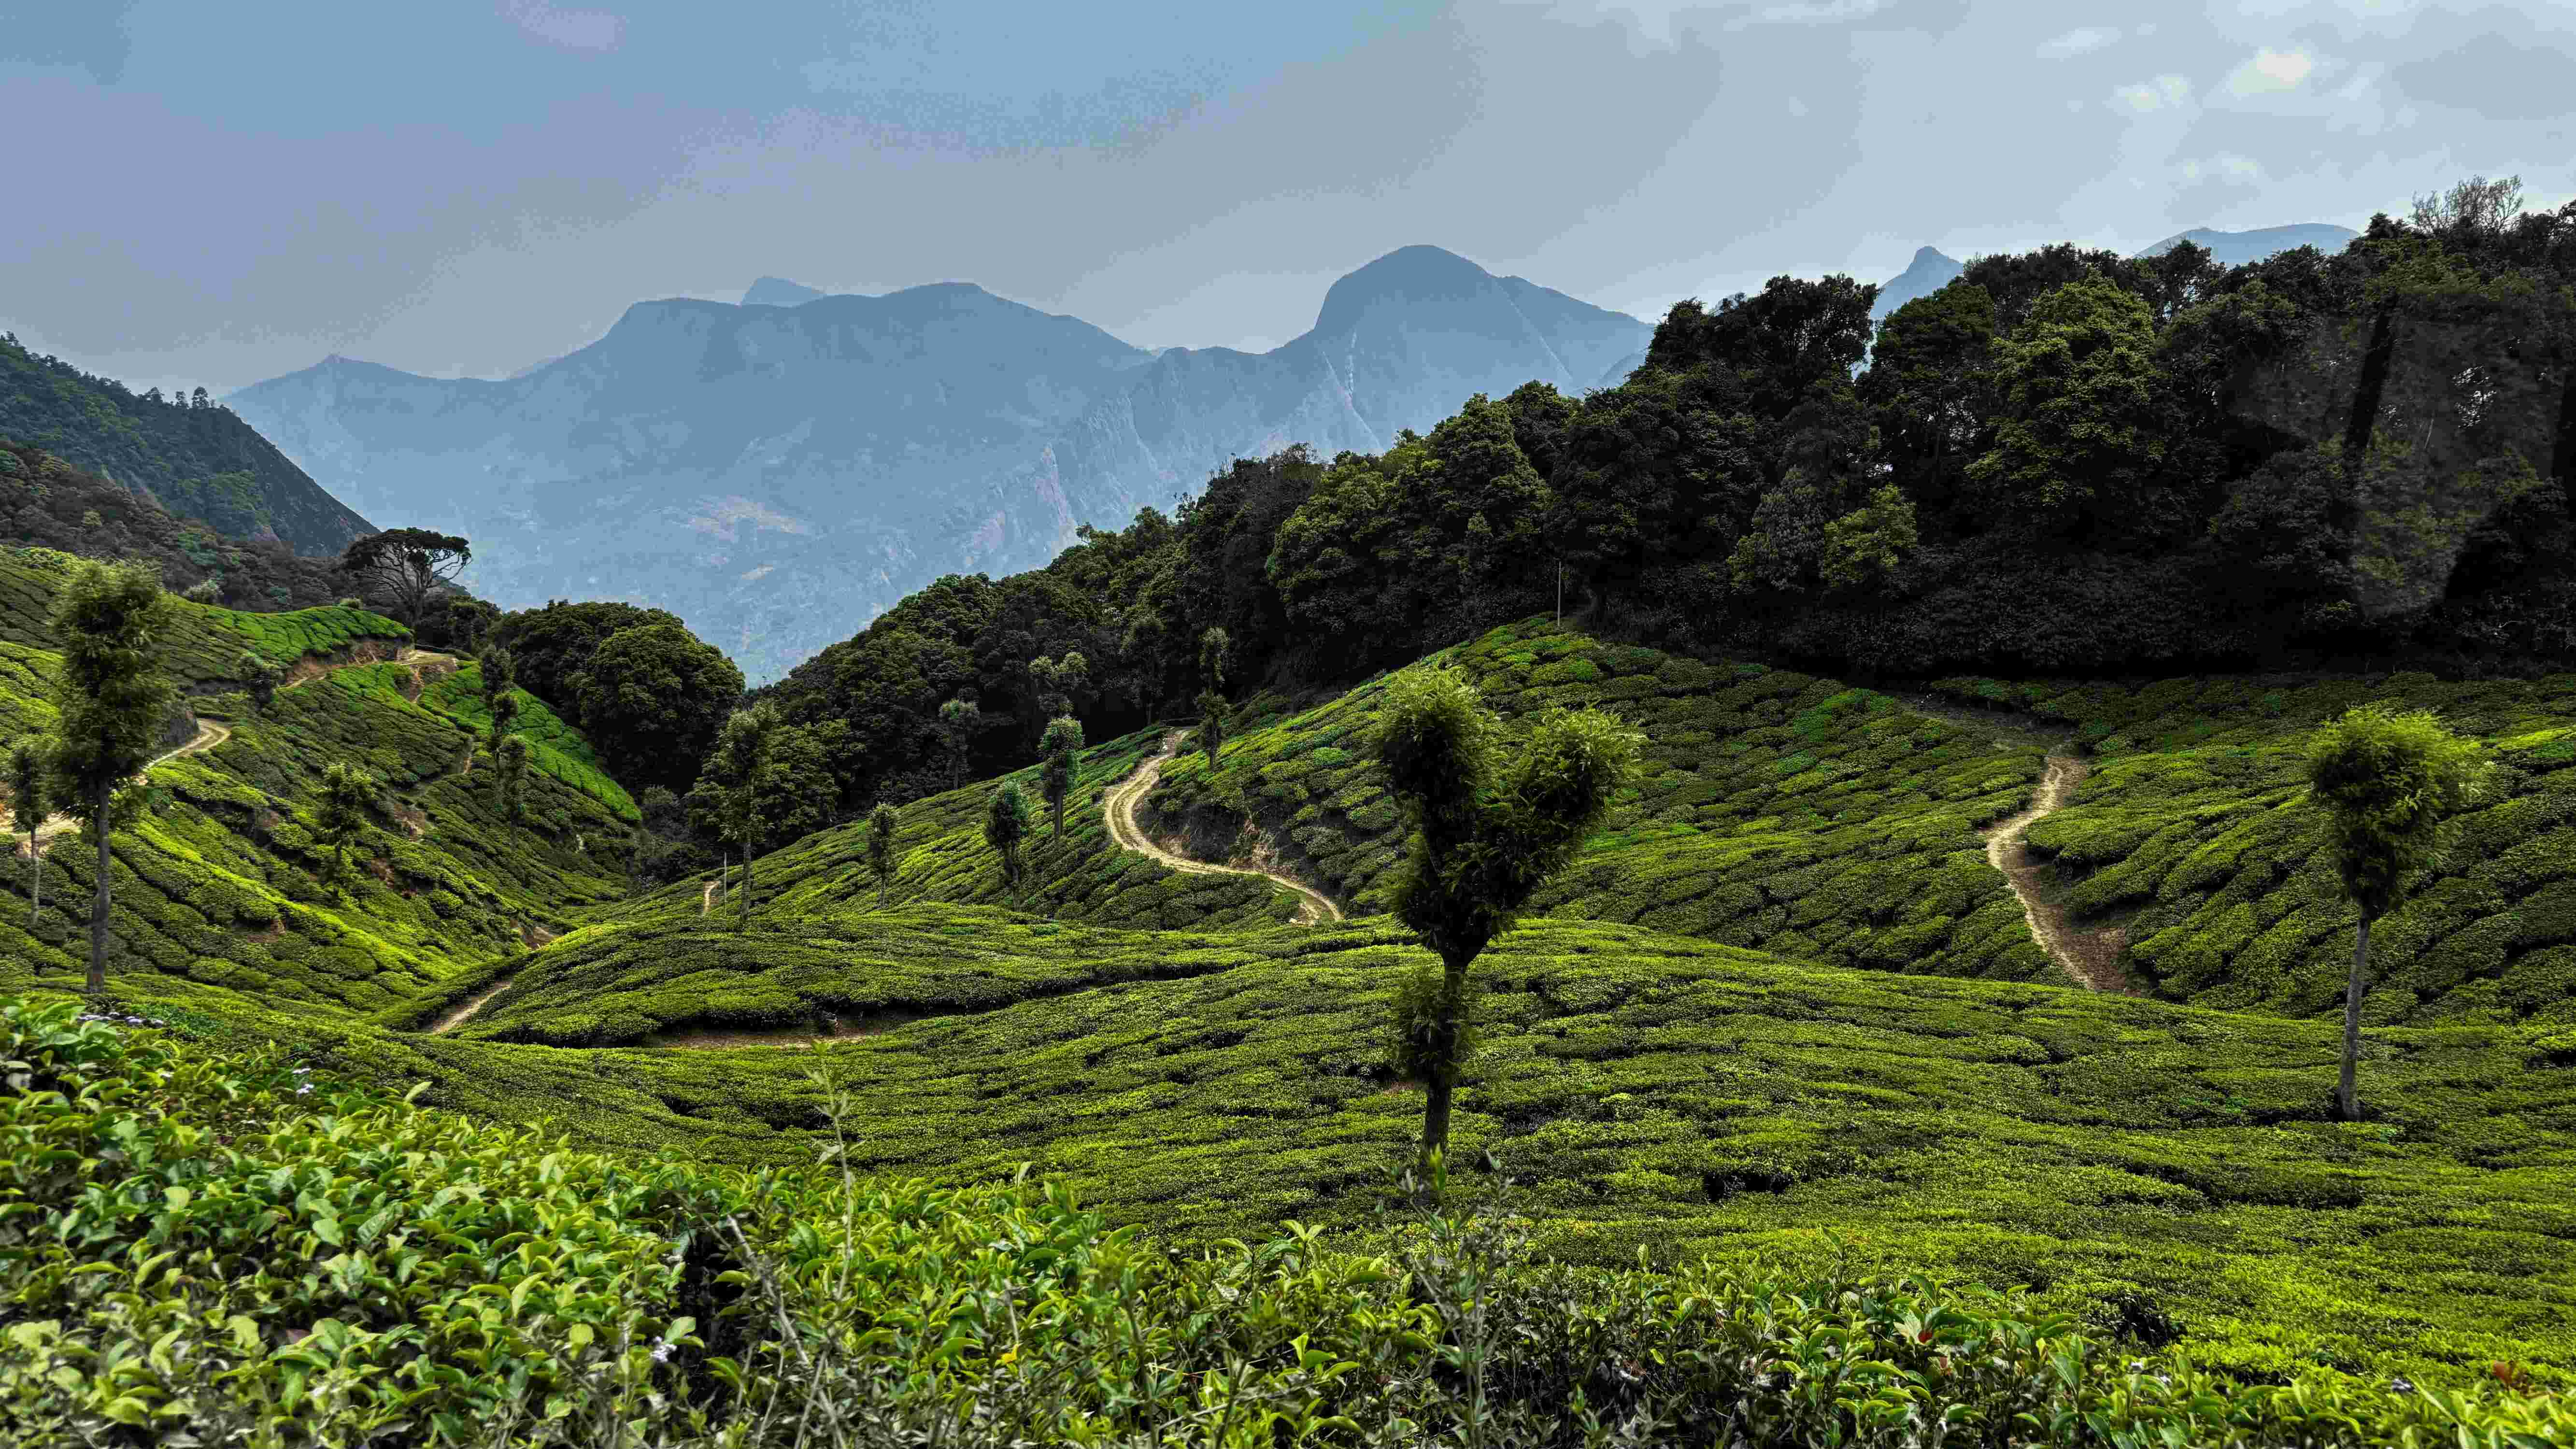
\includegraphics[width=.9\textwidth]{figs/cas-munnar-2024.jpg}
	\caption{The beauty of Munnar, Kerala. (See also Table \protect\ref{tbl1}).}
	\label{FIG:2}
\end{figure*}


\section[Enumerated ...]{Enumerated and Itemized Lists}
{cas-dc.cls} provides an extended list processing macros
which makes the usage a bit more user friendly than the default
\LaTeX{} list macros.   With an optional argument to the
\verb+\begin{enumerate}+ command, you can change the list counter
	type and its attributes.
	
	\begin{verbatim}
		\begin{enumerate}[1.]
			\item The enumerate environment starts with an optional
			argument `1.', so that the item counter will be suffixed
			by a period.
			\item You can use `a)' for alphabetical counter and '(i)' 
			for roman counter.
			\begin{enumerate}[a)]
				\item Another level of list with alphabetical counter.
				\item One more item before we start another.
				\item One more item before we start another.
				\item One more item before we start another.
				\item One more item before we start another.
			\end{verbatim}
			
			Further, the enhanced list environment allows one to prefix a
			string like `step' to all the item numbers.  
			
			\begin{verbatim}
				\begin{enumerate}[Step 1.]
					\item This is the first step of the example list.
					\item Obviously this is the second step.
					\item The final step to wind up this example.
				\end{enumerate}
			\end{verbatim}
			
			\section{Cross-references}
			In electronic publications, articles may be internally
			hyperlinked. Hyperlinks are generated from proper
			cross-references in the article.  For example, the words
			\textcolor{black!80}{Fig.~1} will never be more than simple text,
			whereas the proper cross-reference \verb+\ref{tiger}+ may be
			turned into a hyperlink to the figure itself:
			\textcolor{blue}{Fig.~1}.  In the same way,
			the words \textcolor{blue}{Ref.~[1]} will fail to turn into a
			hyperlink; the proper cross-reference is \verb+\cite{Knuth96}+.
			Cross-referencing is possible in \LaTeX{} for sections,
			subsections, formulae, figures, tables, and literature
			references.
			
			\section{Bibliography}
			
			Two bibliographic style files (\verb+*.bst+) are provided ---
			{model1-num-names.bst} and {model2-names.bst} --- the first one can be
			used for the numbered scheme. This can also be used for the numbered
			with new options of {natbib.sty}. The second one is for the author year
			scheme. When  you use model2-names.bst, the citation commands will be
			like \verb+\citep+,  \verb+\citet+, \verb+\citealt+ etc. However when
			you use model1-num-names.bst, you may use only \verb+\cite+ command.
			
			\verb+thebibliography+ environment.  Each reference is a\linebreak
			\verb+\bibitem+ and each \verb+\bibitem+ is identified by a label,
			by which it can be cited in the text:
			
			\noindent In connection with cross-referencing and
			possible future hyperlinking it is not a good idea to collect
			more that one literature item in one \verb+\bibitem+.  The
			so-called Harvard or author-year style of referencing is enabled
			by the \LaTeX{} package {natbib}. With this package the
			literature can be cited as follows:
			
			\begin{enumerate}[\textbullet]
				\item Parenthetical: \verb+\citep{WB96}+ produces (Wettig \& Brown, 1996).
				\item Textual: \verb+\citet{ESG96}+ produces Elson et al. (1996).
				\item An affix and part of a reference:\break
				\verb+\citep[e.g.][Ch. 2]{Gea97}+ produces (e.g. Governato et
				al., 1997, Ch. 2).
			\end{enumerate}
			
			In the numbered scheme of citation, \verb+\cite{<label>}+ is used,
			since \verb+\citep+ or \verb+\citet+ has no relevance in the numbered
			scheme.  {natbib} package is loaded by {cas-dc} with
			\verb+numbers+ as default option.  You can change this to author-year
			or harvard scheme by adding option \verb+authoryear+ in the class
			loading command.  If you want to use more options of the {natbib}
			package, you can do so with the \verb+\biboptions+ command.  For
			details of various options of the {natbib} package, please take a
			look at the {natbib} documentation, which is part of any standard
			\LaTeX{} installation.
			
			\appendix
			\section{My Appendix}
			Appendix sections are coded under \verb+\appendix+.
			
			\verb+\printcredits+ command is used after appendix sections to list 
			author credit taxonomy contribution roles tagged using \verb+\credit+ 
			in frontmatter.
			
			\printcredits
			
			%% Loading bibliography style file
			%\bibliographystyle{model1-num-names}
			\bibliographystyle{cas-model2-names}
			
			% Loading bibliography database
			\bibliography{cas-refs}
			
			
			%\vskip3pt
			
			\bio{}
			Author biography without author photo.
			Author biography. Author biography. Author biography.
			Author biography. Author biography. Author biography.
			Author biography. Author biography. Author biography.
			Author biography. Author biography. Author biography.
			Author biography. Author biography. Author biography.
			Author biography. Author biography. Author biography.
			Author biography. Author biography. Author biography.
			Author biography. Author biography. Author biography.
			Author biography. Author biography. Author biography.
			\endbio
			
			\bio{figs/cas-pic1}
			Author biography with author photo.
			Author biography. Author biography. Author biography.
			Author biography. Author biography. Author biography.
			Author biography. Author biography. Author biography.
			Author biography. Author biography. Author biography.
			Author biography. Author biography. Author biography.
			Author biography. Author biography. Author biography.
			Author biography. Author biography. Author biography.
			Author biography. Author biography. Author biography.
			Author biography. Author biography. Author biography.
			\endbio
			
			\bio{figs/cas-pic1}
			Author biography with author photo.
			Author biography. Author biography. Author biography.
			Author biography. Author biography. Author biography.
			Author biography. Author biography. Author biography.
			Author biography. Author biography. Author biography.
			\endbio
			
		\end{document}
		
